\documentclass{report}
\usepackage[english]{babel}
\usepackage{microtype}
\usepackage{amsmath,amssymb}
\usepackage{amsthm}
\usepackage[round, authoryear]{natbib}
\usepackage[all]{xy}
\usepackage{graphicx}
\usepackage{framed}
\usepackage{enumerate}
\usepackage{qtree}
\usepackage{mdframed}
\usepackage{tikz}
\usepackage{tikz-dependency}
\usepackage{algorithmic}
\usepackage{algorithm}
\usepackage{float}
\usepackage[OT2,T1]{fontenc}
\newcommand\textcyr[1]{{\fontencoding{OT2}\fontfamily{wncyr}\selectfont #1}}
\newcommand{\myparagraph}[1]{\paragraph{#1}\mbox{}\\}
\bibliographystyle{plainnat}
\renewcommand\topfraction{0.85}
\renewcommand\bottomfraction{0.85}
\renewcommand\textfraction{0.1}
\renewcommand\floatpagefraction{0.85}
\author{}
\title{}

%Define theorem style for definition and metric
\theoremstyle{definition}
\newtheorem{metric}{Metric}
\newtheorem{notion}{Notion}
\theoremstyle{plain}
\newtheorem{definition}{Definition}
\def\citepos#1{\citeauthor{#1}'s (\citeyear{#1})}

%Define new float environment for tables that is boxed
\floatstyle{boxed}
\newfloat{tab}{tbp}{lop}
\floatname{tab}{Table}


\begin{document}

\tableofcontents

%%%%%%%%%%%%%%%%%%%%%%%%%%%%%%%%%%%%%%%%%%%%%%%%%%%%%%%%%%%%%%%%%%%%%%%%%%%%%%%
% INTRODUCTION
%%%%%%%%%%%%%%%%%%%%%%%%%%%%%%%%%%%%%%%%%%%%%%%%%%%%%%%%%%%%%%%%%%%%%%%%%%%%%%%

\chapter{Introduction}

%twee keer something?
Language and meaning play an important role in many aspects of our lives. When means of transportation and communication over larger distances became more publicly available, contact with other cultures became more prevalent and being able to understand how meanings are expressed in other languages than your mother tongue more important. Translation has something intriguing, as it seems to touch on something that is universal for all human beings, but is yet, even for human beings, a very nontrivial task. We would like to start this thesis with a famous quote of Warren Weaver, that we believe has, besides the author of current work, inspired many to pursue a career in machine translation:

\begin{quote}
\textit{``When I look at an article in Russian, I say: `This is really written in English, but it has been coded in some strange symbols. I will now proceed to decode.''} \citep{weaver1955translation}
\end{quote}

Evidently, automatic translation is not as easily solved as Weaver thought at the time. Over 60 years later, the state-of-the-art systems are still not able to produce translations of arbitrary pieces of text with a quality comparable to that of a human translation. This was not for the lack of trying: on Google Scholar one can found over 100,000 articles that contain the phrase ``Machine Translation'', of which almost 10,000 were published in the last two years.

Many different methods have been explored in these articles, one of which is called the transfer method. Contrary to more direct approaches that treat sentences as structureless sequences that can be translated into a sequence of words in another language more or less word for word, the transfer method aims to find structural representations for sentences in the source and target languages and finding a mapping between them. The translation process then consists of analysing the source sentence into a structure, mapping this structure to a target side structure, and generating a target sentence from this structure. A graphical representation of this process is shown in Figure \ref{fig:triangle}. The depicted pyramid shows that direct (word for word) translation can be seen as an extreme of the transfer method, in which the distance from the sentences to the intermediate representation is zero, and thus no analysis or generation takes place. On the other end of the spectrum we can find the case in which the intermediate representation is a universal one, independent of source and target language, and the mapping is the identity mapping. Such a universal intermediate representation of language is called an `interlingua'. 


\begin{figure}[!ht]
\centering
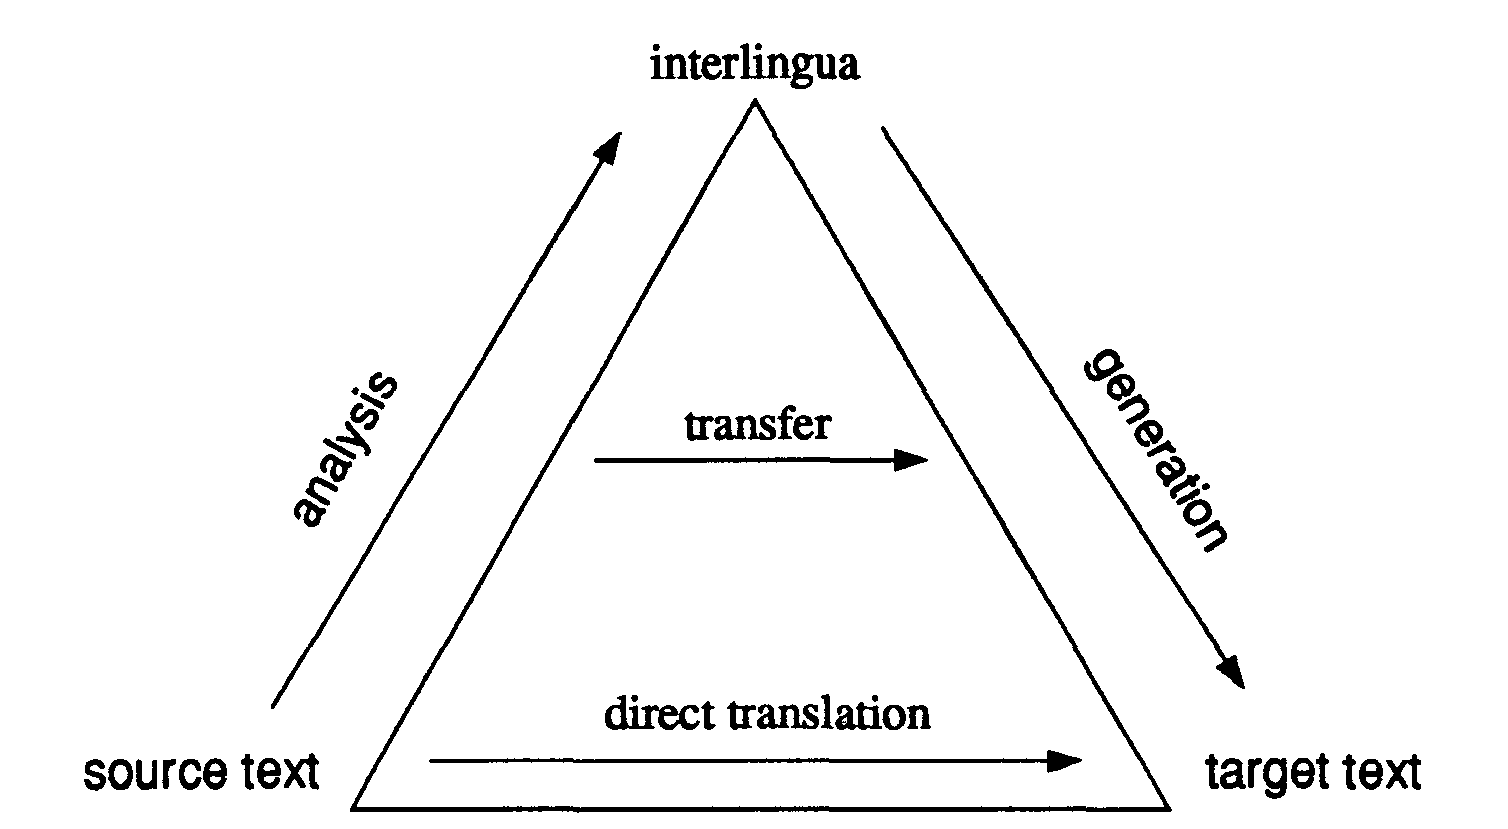
\includegraphics[scale=0.2]{translation_triangle.png}
\caption{Vauquois pyramid?}\label{fig:triangle}
\end{figure}

The pyramid also shows that transfer can be employed in many ways, varying the distance from intermediate representation to source and target language (analysis and generation, respectively). In this thesis, we consider the case in which the intermediate representations are interpreted as structural descriptions specifying how to derive the meaning of a sentence.\footnote{Theoretically, we believe this is the only interesting case of transfer, although transferring other types of information might be useful in practice} In other words, the underlying system generating these structures can be seen as a semantically motivated syntax of the language that specifies how the sentence was (compositionally) constructed with respect to its meaning. Hereby, it is important to notice that such a grammar is recursive, and the mapping between two of such grammars utilizing this fact can thus also be seen as compositional.

This type of transfer is theoretically interesting, as it addresses translation on a very fundamental level. However, although very many translation models have tried to incorporate transfer \citep[e.g.,][]{wu1997stochastic,chiang2005hierarchical}, and compositional methods of translation are theoretically well studied \citep[e.g.,][]{janssen1996compositionality}, it is not fully understood if translation from natural language to natural language can be treated in such a compositional fashion. In translation between other domains (logical languages, programming languages), compositional translation is almost trivially a sound approach, as the expressions of such languages are completely unambiguous and the compositional grammar according to which the meaning can be derived is known. Natural language has neither of these qualities, which does not only complicate the construction of a translation system, but also renders the existence of such a system uncertain.

In practice, the soundness of the approach can only be confirmed - by a machine successfully carrying out translation - and not refuted. Although many researchers have tried, the MT world is far from presenting such a machine. In theory, contrary to in practice, the soundness of the approach can only be refuted - by finding examples that can not be translated as such - and not confirmed. However, it turns out that theoretical examples of non-compositional translations (e.g., idiomatic translations), can often be dealt with elegantly in practice \citep{janssen1996compositionality}. Neither of these approaches thus seem to be promising with respect to determining whether it is possible to systematically construct structures for two languages and a mapping between them.

Nowadays, the availability of huge parallel corpora with texts that are manual translations of each other, together with techniques to align these corpora on the sentence and even word level, provide the means for a different approach. The alignments specify, on different levels of granularity, which units are each others translation and can therefore be interpreted as constraints on the structures possibly used in translation. In this thesis, we will empirically investigate how well these constraints, and the set of structures they give rise to, cohere with linguistic intuitions about language.

Other studies that empirically investigated the properties of translation data through alignments have focussed on the coverage of binary structures \citep[e.g.,][]{sogaard2009empirical1} and the extent to which conventional linguistic syntax oversteps the constraints set by alignment \citep[e.g.,][]{fox2002phrasal,hwa2002evaluating}. The latter studies show that monolingual syntax on its own is not suitable to deliver structures usable in translation, while the former studies provide formal information on the complexity of the reordering phenomena, but do not aim for a linguistic analysis of the multiple structures that can possibly be assigned to a sentence. 

In this thesis, we aim for a more general empirical approach that addresses both the formal and the linguistic side of the problem. We will do so by considering \textit{all} structures describing how a sentence could have been compositionally constructed that are in agreement with the alignment\footnote{As defined in \cite{simaan2013hats}}
(i.e., the set of structures that allow a compositional translation of the sentence), and aim to find one structure for each sentence, such that the resulting set of structures is consistent over the entire corpus, i.e., there is a systematicity in how the structures were derived. As we would like to link this systematicity to linguistic intuitions, we will consider the predicate-argument structures of the sentences as a starting point in this search. As they are closely related to the meaning of the sentence, we believe these structures have potential for being universal for language, and for largely agreeing with alignments. We will investigate how well these structures cohere with predicate argument structures, and analyse the causes in which they deviate from each other.

The contributions of this paper are thus twofold. Firstly, we will investigate the preservation of predicate argument structures across different language pairs. As this yields an empirical view on the universality of such structures, this is interesting for the field of linguistics in general. Secondly, we will aim to devise a method to enrich translation corpora with recursive translation structures based on linguistic intuitions, and shed a light on the difficulties that arise in doing so. The latter is interesting for the field of machine translation, most clearly because it broadens the perspective on the sufficiency of the transfer method, to which it is directly related. Furthermore, a structurally consistent treebank for a parallel corpus might serve as a starting point for a new MT model, and the open source implementation produced for this thesis could prove useful for developing one.


\section*{Thesis Outline}



%%%%%%%%%%%%%%%%%%%%%%%%%%%%%%%%%%%%%%%%%%%%%%%%%%%%%%%%%%%%%%%%%%%%%%%%%%%%%%%
% BACKGROUND MT
%%%%%%%%%%%%%%%%%%%%%%%%%%%%%%%%%%%%%%%%%%%%%%%%%%%%%%%%%%%%%%%%%%%%%%%%%%%%%%%


\chapter{Machine Translation}


%Heb het gevoel dat dit nog herschreven moet worden
In this thesis, we attempt to address the universal properties of language on an empirical level, through studying translation data. On some level, this thesis is thus related to linguistics in general, but the research field to which the thesis is closest, is machine translation (MT). Not only do we build on previous MT research, we also use the corpora, techniques and tools from this field and the results are closely linked with one type of MT models. To fully understand this thesis, it is important to have a basic knowledge of these tools, techniques, and models. This first chapter is intended to make the reader familiar with these.

We will start by briefly describing the development of the fields since the very first attempts, exemplifying the cycle apparent in the types of models that have been investigated. This history will superficial, but rest of the chapter contains more details of models if relevant. References to these sections will be provided in the overview. The history is meant to give an intuitive overview of the developments in MT over the year, we have aimed to keep it short and concise. Hopefully, it will also let the reader appreciate the difficulty of the field, and the number of approaches that have been tried to solve the problem. The difficulty of automatic translation is often underestimated by people not familiar with the field, as translation seems such a natural and human task.

We cannot stress enough that it is not claimed that this chapter provides a complete overview of what has happened in MT over the years. As said, the field is enormous, and in this chapter only a selection is discussed. For instance, neither decoding nor technical implementation details of the models are discussed at all. For more elaborate overviews of MT, the reader can consult \cite{hutchins1992introduction} (early MT), \cite{somers1999review} (exemplar based MT), \cite{koehn2008statistical} or \cite{wu2005mt} (statistical MT), works that have been used as references to write this chapter. The current chapter provides a summary and literature study, but does not present any original work. For readers with an extensive knowledge of MT, it might thus be superfluous.


\section{A brief History of Machine Translation}

Machine Translation arose as a research field almost immediately after the emergence of the first computers. In these early days, several different approaches were explored. 

\myparagraph{Direct Translation}
One branch of research approached translation as encoding, such models with a direct approach to translation are now known as the first generation models. Sentences were translated more or less word for word using some contextual information. Figure \ref{fig:georgetown} contains an example of the translation of the words `much' and `many' into Russian, according to one of the early systems \citep{dostert1955georgetown}.

\begin{figure}[!ht]
\begin{framed}
\footnotesize{
\begin{enumerate}
\item[1] Is the preceding word \textit{how}? (yes $\rightarrow$ \textcyr{skol\char126 ko}, no $\rightarrow$ 2)
\item[2] Is the preceding word \textit{as}? (yes $\rightarrow$ \textcyr{stol\char126 ko qe}, no $\rightarrow$ 3)
\item[3] Is current word \textit{much}? (yes $\rightarrow$ 5, no $\rightarrow$ 6)
\item[4] Not to be translated
\item[5] Is preceding word \textit{very} (yes $\rightarrow$ 4, no $\rightarrow$ \textcyr{mnogo})
\item[6] Is preceding word a preposition, and following word a noun? (yes $\rightarrow$ \textcyr{mnogii}, no $\rightarrow$ \textcyr{mnogo})
\end{enumerate}
}
\end{framed}
\caption{Translation of much and many from English to Russian in a direct translation system. Source: \cite[p.56]{hutchins1992introduction}.}\label{fig:georgetown}
\end{figure}

\myparagraph{Structure Based Translation}
A second line of research followed a more theoretical approach, involving fundamental linguistic research. The models of this strand targeted at translating language making use of its underlying structure. The most ambitious approaches aimed at finding representational systems, called interlingua, to express meaning on an abstract level and translate via such abstract meaning representations (thus finding an abstract meaning representation for the source text and generating a target text from this representation). The results of such models were disappointing, and the general consensus in the MT community was that the less ambitious transfer approach, in which different structural representations for source and target language were used, had the best prospects for significant improvements. In such transfer models, an extra stage is added to the process: the source text is first analysed into a structural representation containing information about the meaning and structure of the text and then this representation is mapped to a target side representation from which a target text can be generated. An example of a transfer rule used in the system Ariane (ref), is depicted in Figure \ref{fig:transferex}.

%better placement of arrow
\begin{figure}
\begin{framed}
\begin{tabular}{lcr}
\Tree [.\textit{supply} [.ARG0\\subj A ] [.ARG1\\obj B ] [.ARG2\\prep-obj \textit{with} C ] ] & $\rightarrow$ & \Tree [.\textit{fournir} [.ARG0\\subj A ] [.ARG2\\i-obj B ] [.ARG3\\d-obj C ] ]\\
\end{tabular}
\end{framed}
\caption{Transfer rule that accounts for the translation of `A supplies B with C' into `A fournit C a B' (accenten)}\label{fig:transferex}
\end{figure}

Although such systems were sometimes successful in small subdomains of language (e.g., \cite{chandioux1976meteo} for meteorolocial forecasts), they failed to scale to bigger domains, as it is very hard to formalize all of language in one system. Driven by exactly this thought, a new line of research came of the ground, that was not primarily based on linguistic knowledge, but on large pairs of texts that were translations of each other.\footnote{Such parallel texts were not created for this purpose, but exist by the grace of multilingual societies. Parallel corpora can be created from, e.g., proceedings of governments that are kept in two languages, websites that are translated into multiple languages, and news organisations that publish their articles for   a multilingual audience \citep{koehn2008statistical}. Techniques to align these text on the sentence level (ref?) have made such parallel texts very valuable for MT research} Corpus based models can be roughly divided into exemplar based models and statistical models. 

\myparagraph{EBMT}
Exemplar based machine translation (EBMT) is directly based on analogy: sentences are translated by finding examples in the corpus similar to (fragments of) the sentence, and generate a translation by recombining them. Although this is very valid as a general idea, such a match-and-change method is computationally not scalable, as huge databases need to be searched for similar phrases or sentences, and similarity is not easy to establish. To exploit the systematicity in translation of natural language, more sophisticated methods are required.

\myparagraph{Statistical Word-based Models}
The first working statistical models \citep{brown1988statistical,brown1990statistical,brown1993mathematics} however, were ground-breaking. Although they were intrinsically word-based, their quality of their translations was an enormous improvement over any earlier model,(?). Equally important is, that the models, now known as `IBM model 1-5', were able to output a translation for any given input sentence (even ungrammatical ones). The statistical framework, that we will discuss more elaborately in Section \ref{sec:IBM}, takes the view that every sentence $t$ is a possible translation of every sentence $s$. Modelling translation thus consists of modelling the probability $P(t|s)$ that $t$ is a translation of $s$, and finding the sentence $t$ for which this probability is highest. The probability distribution is learned using statistical methods, which is where the parallel corpus comes into play. A more detailed description of the models, as well as information on how they deal with phenomena as reordering, can be found in Section \ref{sec:IBM}.

\myparagraph{Statistical Phrase-based Models}
The statistical IBM models still had the same drawbacks as the first generation of direct translation models: no structure or local context was considered, and a large amount of natural language phenomena could therefore not be accounted for. With the introduction of phrases as basic units in translation models \citep{wang1998grammar,och1999improved} a major leap forward was taken towards a proper treatment of these problems. A phrase translation pair is a pair of contiguous source and target sequences such that the words in the source phrase are aligned only with words in the target phrase, and vice versa \citep{och2000improved}. Phrases are thus not restricted to linguistic phrases, but can be any arbitrary contiguous sequence of words whose translation constitutes a contiguous sequence in the target sentence. Phrase-based translation models can therefore capture short contiguous idomatic translations, as well as small insertions and deletions and local reordering. 
%Misschien moet dit stuk verplaatst worden naar de sectie over phrase based translation models??
E.g., both `a casa' and `o casa' are reasonable word for word translations of the English phrase `the house'. However, `o casa' is not a grammatical string in Portugese. The latter observation could be easily captured by a phrase-based model, as `the house' could be translated as one unit, but would be much harder to model in a word-based model. Furthermore, a word-based model would never be able to get the correct idiomatic translation of `kick the bucket' (find other example!), while a phrase-based model would have little trouble finding this translation, provided this specific idiomatic phrase was present in the training corpus. Phrase based models are discussed in more detail in Section \ref{sec:pbmodels}.

\myparagraph{Statistical Structure based Translation Models}
Phrase based models, although still considered state of the art, suffer from the fact that no structure beyond the phrase level is taken into account. Approaches that addressed this problem by incorporating syntactic information to, e.g., sophisticate phrase selection of a standard phrase-based system \citep{koehn2003statistical} or rerank its output \citep{och2004alignment} were not very successful, which lead a large part of the MT community to move back to models similar to the earlier transfer based models that ruled the field before the emergence of statistical models. A major difference with the older transfer models, however, is that the newer models stayed true to the statistical and corpus based tradition, in which translation was formulated as learning a probability distribution from a parallel corpus. While the rules in the old transfer models were constructed manually, the new batch of transfer models were based on the patterns found in translation corpora, making the models more scalable and robust.

\begin{figure}
\centering
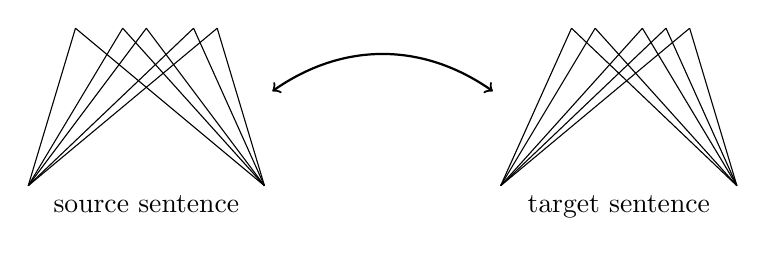
\begin{tikzpicture}

\coordinate (ss) at (1.5,0);
\node [below] at (ss) {source sentence};

%\draw[] (0,0) -- node[below]{source sentence} (3,0);
\draw (0,0) -- (0.6,2) (3,0) -- (0.6,2);
%\draw (0,0) -- (0.9,2) (3,0) -- (0.9,2);
\draw (0,0) -- (1.2,2) (3,0) -- (1.2,2);
\draw (0,0) -- (1.5,2) (3,0) -- (1.5,2);
%\draw (0,0) -- (1.8,2) (3,0) -- (1.8,2);
\draw (0,0) -- (2.1,2) (3,0) -- (2.1,2);
\draw (0,0) -- (2.4,2) (3,0) -- (2.4,2);

\coordinate (ts) at (7.5,0);
\node [below] at (ts) {target sentence};

%\draw (6,0) -- (0.6,2) (9,0) -- (6.6,2);
\draw (6,0) -- (6.9,2) (9,0) -- (6.9,2);
\draw (6,0) -- (7.2,2) (9,0) -- (7.2,2);
%\draw (6,0) -- (7.5,2) (9,0) -- (7.5,2);
\draw (6,0) -- (7.8,2) (9,0) -- (7.8,2);
\draw (6,0) -- (8.1,2) (9,0) -- (8.1,2);
\draw (6,0) -- (8.4,2) (9,0) -- (8.4,2);

\coordinate (startarrow) at (3.1,1.2);
\coordinate (endarrow) at (5.9,1.2);

\draw[<->,bend left =35, thick] (startarrow) to (endarrow);

\end{tikzpicture}
\caption{A graphical representation of compositional translation, or tree-based transfer translation. From a set of possible structures on the source and target side, two suitable structures need to be picked, such that a mapping between them can be created (anders)}\label{fig:comptrans}
\end{figure}

Translation structures, however, are yet another hidden component in translation data. They need to be inferred (or learned), which is a task that is not trivial at all. Some approaches tried to base the structures involved in translation on monolingual syntactic structures, by first parsing the source and target sentence into such a structure, and try to establish correspondences between their nodes. This so called `parse-match-parse' method has a couple obvious limitations. Fully automated parsers that can parse large amounts of text efficiently are required for both source and target language, which extremely limits the amount of language pairs that can be treated with this approach. Furthermore, monolingual grammars are not designed for translation purposes, and there is no guarantee that source and target structures are similar enough to find correspondences for every part of them. This matter will be extensively discussed in Chapter ...

A second approach is to forget about linguistic information, and concentrate on the structures suggested by the translation data. Models using this strategy are based solely on alignments (see \ref{sec:alignments}), which describe which source words are translated into which target words, and the restrictions they impose on structural representations of the sentence (see Chapter ...). As alignments generally give rise to a huge number of rules for every sentence, models using this method are hindered by computational issues. Several different solutions to restricting the rule space have been presented, in some of which formal criteria were used, while in others linguistic information was incorporated. We will discuss these methods in Section \ref{sec:SCFGs}. In this section we will also pay more attention to the practical side of such models.

\myparagraph{Current State of the Art}
Something about what is anno 2013 considered state of the art?

\section{IBM models}
\label{sec:IBM}

In this section, a explanation of the main concepts used in the word-based models presented by \cite{brown1993mathematics} will be provided. These models, that were the first working statistical models, laid the foundation for current state of the art translation models. The IBM-models focussed on learning the probability distributions $P(t|s)$ - the probability that a target sentence $t$ is a translation of a source sentence $s$ - from a parallel corpus. That is, the predefined model for $P(t|s)$ has parameters that can be estimated from the translation data\footnote{For instance, $P(t|s)$ might be dependent on the probability distribution of the translation of the word `obvious' in the corpus.} The hope is, that the learned distribution coincides with human intuitions about translation. For instance, $P(t|s)$ should be high for ($t,s)$ = (`I grow chilli plants in my backyard', `ik kweek chili plantjes in mijn achtertuin'), and low for ($t,s$)= (`I grow chilli plants in my backyard',`gisteren is mijn portemonnee gestolen').

\myparagraph{Modelling $\mathbf{P(t|s)}$}
\citeauthor{brown1988statistical} use Bayes' rule to split the translation probability into multiple probability distributions, yielding the following expression:

\[
P(t|s) = \frac{P(t)P(s|t)}{P(s)}
\]

As $P(s)$ does not depend on $t$, this results in the following equation (called `The Fundamental Equation of Machine Translation' by the authors) for the desired translation $\hat{t}$:

\[
\hat{t} = \operatorname*{arg\,max}_t P(t)P(s|t)
\]

The equation splits the translation task in two: modelling the translation probability $P(s|t)$, and modelling the language probability $P(t)$. In \cite{brown1993mathematics}, 5 different models of increasing complexity are presented to model the translation probability. These models are generally referred to with the names `IBM models 1-5'. In all these models, the probability $P(s|t)$ is modelled by marginalizing over all possible ways in which the words in $t$ could have been generated by the words in $s$, which is expressed by an alignment function $a$ (more information on which can be found in Section \ref{sec:alignments}). Thus: $P(s|t) = \sum_a P(s,a|t)$. $P(s,a|t)$ cannot be computed exactly, and the 5 IBM models differ in the complexity of their approximation. For instance, in IBM model 1, all alignments are assumed to have an equal probability, and the probability $P(s,a|t)$ is the (normalized) product of all the lexical translation probabilities $p(s_j|f_{t(j)})$ indicated by the alignment. The translation probabilities for sentences $t$ with the same words in different orders are thus identical. To address this issue, an alignment probability distribution is added in IBM model 2. In later models, also fertility of the input words is considered, and the distortion model is made more sophisticated. In Figure \ref{fig:IBM-model} an example of IBM-style translation is depicted. The parameters of the IBM models (e.g., lexical translation probabilities, fertilities of the words, alignment probabilities) are learnt from a parallel corpus using the expectation maximization algorithm \citep{dempster1977maximum}, on which a short explanation can be found in Section \ref{sec:alignments}. Mathematical details on the exact procedure of parameter estimation for the IBM models can be found in \cite{brown1993mathematics}.

\begin{figure}[!ht]
\begin{framed}
\scriptsize{
Consider the following pair of sentences and a possible alignment (the numbers indicate the alignment: (Le chien e battu per Jean, John (6) does beat (3,4) the (1) dog (2)). The probability $P(s,a|t)$ is computed as follows:\begin{enumerate}
\item Compute the lexical probabilities of the source words being translated into the target words, thus compute: $P(Jean|John)\cdot P(est|beat)\cdot P(battu|beat)\cdots$
\item factor in the fertility probabilities of the source words, thus multiply with:  $P(f\!=\!1|John)\cdot \cdot P(f\!=\!1|does) \cdot P(f\!=\!2|beat)\cdots $
\item Factor in the distortion probabilities, that are in this model just depending on source and target position and target length, thus multiply with: $P(1|4,l\!=\!6)\cdot P(2|5,l\!=\!6)\cdot P(3|3,l\!=\!6) \cdots $
\end{enumerate}
The parameters for this IBM model are thus: a set of lexical translation probabilities $P(f|e)$, a set of fertility probabilities $P(n|e)$ and a set of distortion probabilities $P(i|j,l)$ for each target position $i$, source position $j$ and target length $l$. In practice, $i,j,l$ and $n$ are maximally $25$.
}
\end{framed}
\caption{Example from \cite[p.3]{brown1990statistical}, that shows the workings of the IBM word-based translation model}\label{fig:IBM-model}
\end{figure}

The language model, a probability distribution for $P(t)$, is supposed to account for fluency and grammaticality of the target language string. That is, to prevent the model from putting too much probability mass on not well formed target strings. In the IBM models, the probability distribution is an $n$-gram model, whose parameters can be estimated through relative frequency estimation on the target side of the parallel corpus. The set-up in which a separate language model is used to assign probabilities to translations is used by almost every current state of the art MT-model.


\section{Phrase-based models}
\label{sec:pbmodels}

%Explain difference in generative model phrase-based and word-based translation
Using sequences of words as basic units in translation models rather than single words, allows the translation model to take into account local context. For instance, the translation of a sentence with a simple phrase based models could go as follows: the foreign sentence is first broken up into phrases. These phrases are then translated as a whole, and the probability of the source sentence\footnote{A quick reminder: the generative model of phrase-based models is largely similar to the word-based IBM models, the translation probability is still inverted due to application of Bayes' rule.} is defined as the product of the phrasal translation probabilities and distortion based on how far every phrase was moved relatively to the previously translated phrase \citep{koehn2003statistical}. After taking into account the language model, the target sentence with the highest probability $P(t|s)$ can be found. (anders)

To translate with phrases, a phrase translation table is needed in which probabilities are assigned to the translation of source phrases in target phrases. Phrase-tables can be acquired in different ways \citep{marcu2002phrase,och1999improved,koehn2003statistical}, details of which are not relevant to this thesis. More relevant to this thesis is what is means for a phrase to be consistent with the alignment, which we will discuss in Chapter 2.

Phrase-based translation has some obvious advantages over word-based translation. First of all, it can account for short idiomatic translations in an intuitive fashion: directly assigning a probability to `of course' as the translation of `natuurlijk' makes intuitively more sense than having two separate entries for that assign probabilities to `of' and `course' being translations for `natuurlijk'. Secondly, phrases can use local context, which means they can make informed decisions about the translation of, e.g., the gender of determiners and adjectives. Finally, phrases can capture local reordering phenomena of phrases seen during training, making it easier to prefer `the beautiful house' over `the house beautiful' as translation of `la casa bella'.

Phrase based models also have certain limitations, of both practical and theoretical nature. Firstly, when it comes to reordering, phrase based models have no means of generalizing beyond what they have seen in the training data. This means that local reordering of previously mentioned phrases like `la casa bella' can be captured by a phrase-based model if the exact phrase occurred in the training data, but the model will not be able to infer that adjectives and nouns in translation between Italian and English generally switch order. For the same reason, phrase-based models are not able to account for global reordering phenomena, although that is also partly due to the fact that no discontinuous phrases are allowed. A second issue concerns the partitioning of the sentence into phrases. The probability of this partitioning is rarely considered, and phrases are not allowed to overlap, resulting in poor modelling of agreement phenomena. Finally, as mentioned before, assigning probabilities to phrase pairs is not straight forward. Several approaches have been used to learn phrase-translation tables \citep[see][p.130]{koehn2008statistical}.

\section{Synchronous Context Free Grammars}
\label{sec:SCFGs}

To address the global reordering problem, more structure needs to be incorporated, which brings us back to transfer models. For a transfer model that incorporates structure on a more global level, syntactic formalisms for both source and target side are needed, as well as method of combining them. A generative model that is often used in tree-based transfer models is the synchronous grammar, that is assumed to generate source and target sentences simultaneously. The complexity of the monolingual grammars that are linked may differ. Although some translation model have incorporated simpler formalisms \citep[e.g., finite state machines, in][]{alshawi2000learning}, the lion's share of the tree based transfer models use context free grammars (CFG's) \citep{chomsky1956three}. A synchronous context free grammar, assumes that both languages can be modelled by a CFG:


\begin{definition}[Context Free Grammar]
A context free grammar (CFG) is a quadruple $G = (V, \Sigma, R, S)$, where\begin{enumerate}
\item $V$ is a (finite) set of non-terminals, in the context of natural language interpreted as syntactic categories.
\item $\Sigma$ is a (finite) set of terminals, corresponding to the lexical items of the language.
\item $R$ is a relation from $V$ to $V\cup\Sigma$, to be interpreted as a set of rewrite rules.
\item $S\in V$ is a start symbol of the grammar.
\end{enumerate}
\end{definition}

An SCFG \citep{aho1969properties} is a grammar linking two CFG's that share a set of non-terminals, describing how their expressions can be generated simultaneously. Parse trees generated by SCFGs thus need to be isomorphic on the non-terminal level (i.e., there is a bijective mapping between the non-terminal nodes of the trees). Formally, we have:

\begin{definition}[Synchronous Context Free Grammar]
A synchronous context free grammar (SCFG) is a quadruple $G = (V, \Sigma, R, S)$, where\begin{enumerate}
\item $V$ is a (finite) set of non-terminals, the syntactic categories of both languages.
\item $\Sigma$ is a (finite) set of terminals, constituted by the union of the terminal symbols of the two languages.
\item $R$ is a set of rewrite rules of the form $X\rightarrow\langle\gamma,\alpha,\sim\rangle$, $\gamma\in (V\cup\Sigma)^{*}$,  $\alpha\in (V\cup\Sigma)^{*}$ and $\sim$ a one-to-one correspondence between the non-terminal symbols in $\alpha$ and $\gamma$
\item $S\in V$ is a start symbol of the grammar.
\end{enumerate}
\end{definition}

SCFG's implicitly model large scale reordering phenomena and long distance dependencies, as the non-terminal sequences that are generated with every productions do not necessarily have the same order.

\subsection{Difficulties of SCFG's}

As most MT-models, SCFG's are severely hindered by computational problems. Before describing how SCFG's can be learned, we will highlight one of this problems related to the rank of an SCFG, that has been a motivational factor in many algorithms for learning SCFG's. The rank of an SCFG can be defined as the highest number of non-terminals occurring on the right hand side of a rule in the grammar in a single dimension \citep{gildea2006factoring}. As with monolingual CFG's, parsing with SCFG's is much more efficient if all the rules are binary (thus the rank of the grammar is 2). Contrary to monolingual CFG's, the rank of an SCFG can not always be reduced to two by rewriting the rules. That is, synchronous CFG's can not always be binarised \citep{huang2009binarization}. 
Discuss more difficulties?


\subsection{Learning SCFG's}
\label{subsec:learningSCFGs}

SCFG's are very popular as generative model in SMT, even approaches that are not explicitly concerned with them can often be reformulated as such. Learning an SCFG from translation data is a far from trivial task, which is amplified by the fact that bilingual data often do not coincide with monolingual linguistic structures. That is, trees generated by SCFG's are isomorphic on the non-terminal level, which is often not the case if two separate non adjusted parsers are used to generate source and target side trees. Furthermore, the parts considered constituents by a monolingual CFGs are not necessarily translation admissible parts according to the translation data.\footnote{This will be discussed in detail in Chapter 2.} Translation models solely relying on monolingual syntactic structures thus exceed the power of SCFG's, we will briefly discuss them in Section \ref{sec:bcf}.

In almost all working SCFG models, the grammar is induced from a parallel corpus by regarding the data as primary source of information (in contrast to using external (linguistic) knowledge). This approach - introduced by \cite{wu1995algorithm} in the form of an inversion transduction grammar (ITG), that lies at the heart of many later approaches - is based on word-alignments and the constraints on structures they prescribe. In Chapter \ref{ch:empirical}, we will take a closer look at alignments and the structures they induce.

Purely data-driven models reinforce the computational problems of SCFG's, as the number of rules that can be extracted from a sentence grows exponentially with the length of the sentence\citep{quirk2006dependency}. Without considering additional information, there is no a priori reason to prefer one rule over another, yet some serious pruning of the rule space is necessary to make parsing computationally feasible. Furthermore, without linguistic information, a grammar naturally lacks non-terminal labels. Models differ in the number and kind of non-terminal labels that they use. In the remainder of this section we will briefly discuss two strategies that have been proposed to address the previously mentioned issues. The strategies are not mutually exclusive, some models use them both. The explanation is meant to exemplify endeavours to address these problems, and although several references to models are provided it is not meant to give a complete overview of these.
%Maybe say something about other approaches that we won't discuss: log-linear framework, feature based approaches

\subsubsection{Restricting according to Rank}

A remedy that is often used to reduce the number of rules is to select only the rules of which the number of righthand side non-terminals does not exceed a certain maximum number. In most cases, the rules are restricted to binary, which reduces both the rule space and the parsing complexity \citep[e.g,][]{wu1997stochastic,chiang2005hierarchical,mylonakis2011learning}. The solution is thus computationally attractive, and easy to implement. Of course, the assumption that all of language can be captured in binary structures seems rather strong. \citeauthor{wu1997stochastic} claimed to be unable to find real-life examples of translations that could not be explained by such trees, but this was later refuted by others \citep[e.g.,][]{galley2004s}. However, the coverage of binary transduction grammars is still a hot issue in MT, to which we will come back later in Chapter \ref{ch:empirical}. 

Several of the models using this paradigm to prune the rule space do not really address the non-terminal label issue. \citepos{wu1995algorithm} contains only a single non-terminal label, his model thus merely learns a high-level reordering preference, without considering further contextual information. An improvement on this was presented by \cite{chiang2005hierarchical,chiang2007hierarchical}. Although his grammar also had no more than one non-terminal label, he allowed the right-hand side of his rules to contain both terminals and non-terminals, such that lexical information could be incorporated. An example of such a rule would be:

\[
\text{X } \rightarrow \langle\text{ X}_1 \text{ de X}_2 \text{, the X}_2 \text{ that X}_1\rangle
\]

which captures the fact that Chinese relative clauses modify noun phrases on the left, whereas English relative clauses modify on the right \citep{chiang2007hierarchical}.\footnote{To combine different non-terminals into a sentence, some more rules are needed. \cite{chiang2007hierarchical} adds the following two `glue rules' to his grammar:\begin{align*}
 \text{S } \rightarrow \langle\text{ S}_1\text{X}_2 \text{,S}_1\text{X}_2\rangle\\
\text{S } \rightarrow \langle\text{ X}_1 \text{,X}_1\rangle 
\end{align*}

}

The framework introduced by Chiang combines the strengths of rule-based and phrase-based models, and is referred to with the term `Hierarchical Phrase Based Translation'. A model with a similar set-up was presented by \cite{mylonakis2010learning}, who extended a standard HPB model with two extra non-terminal labels to decode whether a phrase-pair tends to take part in other switching. They showed that it is possible to train a complete all-phrase binary grammar with cross validated EM. Besides their model, and the one presented in \cite{blunsom2008bayesian}, there are no other models that learn syntactic categories without invoking linguistic knowledge.


\subsubsection{Incorporating Linguistic Information}

A tangible solution to address the previously mentioned issues with structure-based transfer models is to incorporate linguistic knowledge. Information from monolingual parsers can be used to, e.g., reduce the space of possible node spans, and to induce linguistically motivated terminal labels.

The later was done by, e.g., \cite{zollmann2006syntax} and \cite{almaghout2010ccg}, who augmented a standard phrase-based grammar with syntactically motivated non-terminal labels, based on constituency grammars and ccg \citep{steedman2011combinatory}, respectively. \cite{mylonakis2011learning} learn automatically which source-syntax labels fit best with a phrase-based CFG and the translation data.

Clearly, the number of language pairs that can be treated as such, as it requires an automated linguistic parser (or other means of providing linguistic information on alarge scale) for (at least one of) source and target language. However, using available syntactic or semantic knowledge can result in robust models that yet do not ignore or intuition of language, especially if high quality parsers are available.

Aanvulen met andere modellen?


%Deze sectie moet je echt nog even goed doorlezen en herschrijven!!!!

\section{Beyond Context Free}
\label{sec:bcf}

Formally it is desirable to create grammars that generate isomorphic tree pairs for sentences that are each others translation, but there is no a priori reason that dictates that such structures exist. In fact, as CFG's have been proved to sometimes be inadequate to model certain natural language phenomena, more powerful transformation methods might be suitable for the expressive syntactic transformations going on during the translation of natural language. As the necessity of deviating from conventional syntax is smaller, models of this class tend to stay closer to traditional linguistic structures.

\subsection{Synchronous Tree Substitution Grammars}

The class of Synchronous Tree Substitution Grammars (STSG's) is a strict superset of the class of SCFG's, and STSG's are therefore a natural extension to them. Models working with STSG's are, i.a., \cite{poutsma2000data} and \cite{galley2004s,galley2006scalable}. The core method of the former is to align chunks of parse trees of source and target sentences, and transform them into rules. \cite{poutsma2000data} requires the existence of a parallel corpus aligned on the subtree level. Such datasets were not available and the paper is merely a description of the STSG framework.  The model presented by \citeauthor{galley2004s} has a somewhat different set-up, learning rules to transform an source-language string into a target language tree. \cite{galley2006scalable} does provide an implementation, yielding promising results.\\
An approach that does not explicitly use STSG's, but whose grammar rules do exceed the power of CFG rules, is presented by \cite{melamed2004generalized}. In their generalized multitext grammar (GMTG) they let go of the requirement that constituents need to be contiguous, which allows them to synchronise languages generated by mildly context-sensitive languages. (anders) Also \citeauthor{melamed2004generalized} present a framework with suggestions for further work, rather than an implementation.

\subsection{Semantic Mappings}

The last category of models we will discuss, attempts to find mappings between more semantically oriented structures, that specify the predicate-argument structure of the sentence, that is often assumed to be somewhat universal. Such an approach is taken in \cite{menezes2003best}, in which transfer rules are extracted by aligning pairs of Logical Form structures. Another predicate-argument structure that is often used is the dependency parse (for more information on the dependency parse, see \ref{sec:depgram}), rules are inferred by either projecting or learning target-side paths. As such rules sometimes create or merge dependents according to the alignment, the dependency structures of source and target side need not be isomorphic, and such models can formally also be seen as STSG's (as made explicit in \cite{eisner2003learning}). Finding a mapping between two dependency trees is not only attractive because dependency trees represent the semantic structure of a sentence more closely than a constituency tree, but also because it is computationally more feasible, as dependency trees contain fewer nodes than constituency trees of the same sentence. Presented models differ in the linguistic plausibility of the target side dependency parse. E.g., \cite{eisner2003learning} learns mappings between two dependency trees (his article lacks a working implementation, although it does give a description of algorithms suitable for parsing with his model). \cite{lin2004path}, extracts transfer rules that correspond to linear paths in the source side dependency tree, but not necessarily to linguistic dependency parses on the target side. The models presented in \cite{quirk2005dependency,quirk2006dependency,quirk2006we} also have clear dependency part, but employ several other strategies as well. They project source dependency trees to target dependency trees, following a set of rules, and extract from the resulting corpus a set of \textit{treelets} - arbitrary connected sub graphs - that are used in translation.

 
%%%%%%%%%%%%%%%%%%%%%%%%%%%%%%%%%%%%%%%%%%%%%%%%%%%%%%%%%%%%%%%%%%%%%%%%%%%%%%%
% BACKGROUND EMPIRICAL
%%%%%%%%%%%%%%%%%%%%%%%%%%%%%%%%%%%%%%%%%%%%%%%%%%%%%%%%%%%%%%%%%%%%%%%%%%%%%%%
 
 
\chapter{Empirical Research of Transfer Models}
\label{ch:empirical} 

In the previous chapter, we have given an overview of the applied field of MT, to which this thesis is related. We have provided a short history of MT, we have have mentioned the relevant techniques applied in MT, and we have briefly discussed the different directions that can be followed in designing a transfer model. In this chapter, we will consider transfer models on deeper, more theoretical level and with more technical details. We will tear apart the assumptions underpinning transfer models, discuss their implications for natural language on a theoretical level, and discuss how they could be assessed on an empirical level. This chapter will alternate depth and breadth, to help the reader, we will start with an overview of the contents.

\subsection*{Overview}

In the first two sections of this chapter, we will discuss the two main assumptions underpinning transfer models, that is:

\begin{enumerate}
\item Abstract structures of both languages exist, and hence an underlying system generating such structures.
\item It is possible to systematically map structures from the representational system from one language to the representational system of the other language.
\end{enumerate}

In both sections, we will start with a theoretical discussion of the assumption, on the basis of literature on compositionality. The second part of both sections, addresses the assumptions on a more practical level, by explaining how they can be interpreted in concrete terms. The third section can be seen as an intermezzo in which the two previous chapters are linked, and related to empirical research. In the fourth section, the two transfer assumptions are addressed on an even more concrete level, as the tools directly related to the assumptions are discussed, preparing the reader for the empirical part of this thesis. In the fifth section, we discuss the assumptions and simplifications that are made to conduct empirical research, and pose some concrete questions such research might provide an answer to. We finish by discussing the answers that have already been found in the literature, prior to this thesis.



\section{Structures of Language}

Transfer models require a method for assigning a structural representation to sentences of a language, wherein the meaning is contained. In other words, it is assumed that there is an underlying representational system, according to which a sentence can be parsed. There is no consensus in linguistics as to the existence of such a system. On the one hand, there is the Chomskian group of researchers, that adhere the existence of an underlying compositional grammar universal to all human beings (ref?), while others believe no such system exist, and language users rely on some sense of familiarity with what they have heard before \citep[e.g.,][]{frank2012hierarchical}. However, cognitive considerations are beyond the scope of this thesis. In this section, we will discuss the implications of compositionality of language on a more theoretical level, and explain how it can be tested in practice.

\subsection{Theory}

The stand that language is a compositional system generated by a language is well discussed in the literature. The following theoretical principle captures this property of language:

\begin{quote}
\textbf{The Principle of Compositionality}\\
The meaning of an expression is a function of the meaning of its parts and the syntactic rule by which they are combined \citep{partee1984compositionality}
\end{quote}

The principle applies rather obviously to (most) artificial languages created by humans. The meaning of their expressions can be unambiguously determined by considering the atoms and the rules used to combine them. For instance, consider the expression $p\lor q$ in propositional logic. Its truth-value can be determined by plugging in the truth values of $p$ and $q$ into the rule of the $\lor$-connective. Also programming languages can be interpreted by considering their basic units and the rules used to combine them.

Intuitively, it seems very reasonable that natural languages should obey this principle as well: we do not store the meaning of all possible sentences of language in our head, and yet we have no trouble understanding new sentences, presumably because we know the words in it, and the methods that can be used to combine them. Besides, we can all perceive a certain systematicity and recursion in the way sentences are constructed. However, it is hard to establish the level of compositionality of language as a whole. The difficulty consists of two, not unrelated, issues.

First of all, creating a grammar that covers \textit{all} grammatical utterances of a natural language, without generating too many ungrammatical ones, has proven a far from trivial task. It is surprisingly difficult to construct such a compositional grammar, even for a finite (but reasonably sized) non-trivial corpus \citep{scha1990taaltheorie}. The bigger the grammar grows, the more phenomena need to be taken into account, as well as how they interact with each other. Also, such a grammar should contain all idiomatic expression of the language, whose meaning cannot be derived from its parts.

The second difficulty concerns ambiguity. In programming and logical language, utterances typically have only one analysis, and their meaning is thus unambiguous. Under all current existing grammar formalisms assigning structures to natural language, all sentences (of some length) have many different structural analyses, of which mostly only one or two are perceived by humans \citep{scha1990taaltheorie}. Even sentences that are considered unambiguous by humans thus need to be disambiguated.\footnote{Note that this problem differs from one of the standard counter arguments of compositionality, that concerns sentences like `two men carry two chairs', that \textit{are} considered ambiguous by humans, but cannot be assigned two distinct syntactic analyses capturing this difference \citep{pelletier1994principle}. Not particularly relevant, but certainly nice to notice, is that this type of ambiguity is not necessarily problematic for translation, as it might be preserved. For instance, the Dutch translation `twee mannen dragen twee stoelen' of aforementioned sentence has the same two meanings as the English one.} In practice, this issue is often solved by assigning probabilities to the grammar rules, and computing the structure with the maximum probability (or an approximation of this).

End paragraph with concluding remark

%In summary, without constructing a grammar that generates all and only all utterances of a natural language, it seems impossible to theoretically establish the level of compositionality. 

\subsection{In Practice}

We will now explain how compositional structures are generated, or identified. For the moment, we will not pay any attention to the syntactic rules used in the derivation of a structure, but merely focus on which parts were used during the construction of the sentence. This part of the thesis is very basic, but is very important for the work done in this thesis and will therefore be treated nevertheless.

Consider the simple sentence `I gave my little brother a new toy car.'. There are very many ways, in which this sentence could be built up from its parts, such as:\begin{itemize}
\item combine `brother' and `a' to get `brother a'
\item combine `I', `gave', `my' and `little' to get `I gave my little'
\item combine `new', `toy' and `car' into `new toy car'
\item combine `I gave my little' and `brother a' to get `I gave my little brother a'
\item combine `I gave my little brother a' and `new toy car' to get the entire sentence
\end{itemize}

This construction can be represented in a tree structure, as is depicted in Figure \ref{fig:struct1}.

\begin{figure}[!ht]
\centering
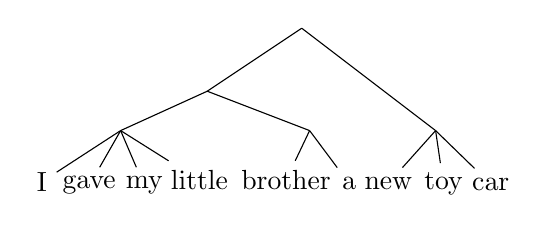
\begin{tikzpicture}
\node (I) at (1,0.05) {I};
\node (gave) at (1.6,0) {gave};
\node (my) at (2.3,0) {my};
\node (little) at (3.0,0.07) {little};
\node (brother) at (4.1,.07) {brother};
\node (a) at (4.9,0.03) {a};
\node (new) at (5.4,0.03) {new};
\node (toy) at (6.1,0.02) {toy};
\node (car) at (6.7,0.02) {car};

\coordinate (Igavemylittle) at (2,0.7);
\coordinate (brothera) at (4.4,0.7);
\coordinate(newtoycar) at (6.0,0.7);
\coordinate (all) at (4.3,2);
\coordinate (Igavemybrothera) at (3.1, 1.2);

\foreach \from/\to in {Igavemylittle/I, Igavemylittle/gave, Igavemylittle/my, Igavemylittle/little, a/brothera, brother/brothera, newtoycar/new, newtoycar/toy, newtoycar/car, Igavemybrothera/Igavemylittle, Igavemybrothera/brothera, all/newtoycar, all/Igavemybrothera}
	\draw (\from) -- (\to);

\end{tikzpicture}
\caption{A tree that describe how the sentence 'I gave my little brother a new toy car' could have been compositionally constructed.}\label{fig:struct1}
\end{figure}

Formally, there is no reason to discard this structure, yet everyone that understands the English language will agree that this structure makes little sense, as we perceive that other parts somehow belong together, such as `my little brother', or `a new toy car'. The structures in Figure \ref{fig:struct2} therefore seem more plausible.

\begin{figure}[!ht]
\centering
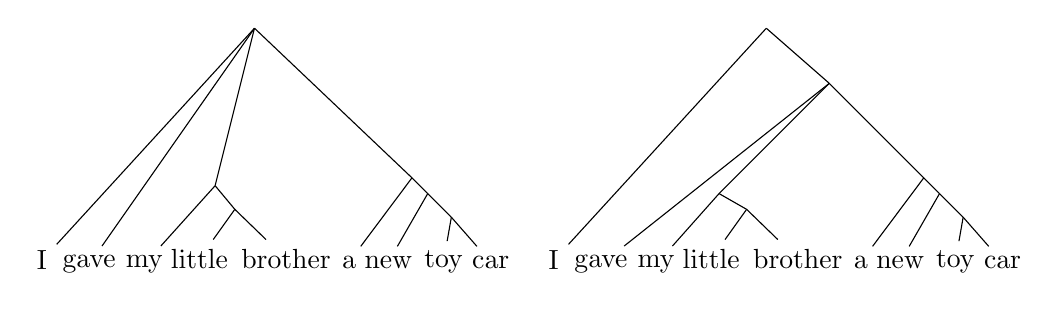
\begin{tikzpicture}

\node (I) at (0,0.05) {I};
\node (gave) at (0.6,0) {gave};
\node (my) at (1.3,0) {my};
\node (little) at (2.0,0.07) {little};
\node (brother) at (3.1,.07) {brother};
\node (a) at (3.9,0.03) {a};
\node (new) at (4.4,0.03) {new};
\node (toy) at (5.1,0.03) {toy};
\node (car) at (5.7,0.03) {car};

\coordinate (toycar) at (5.2,0.6);
\coordinate(newtoycar) at (4.9,0.9);
\coordinate (anewtoycar) at (4.7,1.1);
\coordinate (littlebrother) at (2.45,0.7);
\coordinate (mylittlebrother) at (2.2,1);
\coordinate (all) at (2.7,3);

\foreach \from/\to in {toycar/car, toycar/toy, newtoycar/toycar, newtoycar/new, anewtoycar/newtoycar, anewtoycar/a, littlebrother/brother, littlebrother/little, mylittlebrother/littlebrother, mylittlebrother/my, all/I, all/gave, all/mylittlebrother, all/anewtoycar}
	\draw (\from) -- (\to);

\node (I_) at (6.5,0.05) {I};
\node (gave_) at (7.1,0) {gave};
\node (my_) at (7.8,0) {my};
\node (little_) at (8.5,0.07) {little};
\node (brother_) at (9.6,.07) {brother};
\node (a_) at (10.4,0.03) {a};
\node (new_) at (10.9,0.03) {new};
\node (toy_) at (11.6,0.03) {toy};
\node (car_) at (12.2,0.03) {car};

\coordinate (toycar_) at (11.7,0.6);
\coordinate(newtoycar_) at (11.4,0.9);
\coordinate (anewtoycar_) at (11.2,1.1);
\coordinate (littlebrother_) at (8.95,0.7);
\coordinate (mylittlebrother_) at (8.6,0.9);
\coordinate (gavetobrother_) at (8.1,1.3);
\coordinate (gavetocar_) at (10,2.3);
\coordinate (all_) at (9.2,3);

\foreach \from/\to in {toycar_/car_, toycar_/toy_, newtoycar_/toycar_, newtoycar_/new_, anewtoycar_/newtoycar_, anewtoycar_/a_, littlebrother_/brother_, littlebrother_/little_, mylittlebrother_/littlebrother_, mylittlebrother_/my_, all_/I_, gavetocar_/gave_, gavetocar_/mylittlebrother_, gavetocar_/anewtoycar_, all_/gavetocar_}
	\draw (\from) -- (\to);
\end{tikzpicture}
\caption{Possible compositional structures for the sentence `I gave my little brother a new toy car'}\label{fig:struct2}
\end{figure}

Such tree representations can be used to capture any compositional structure: every node corresponds to the application of a syntactic rule in the derivation, where its children were the arguments. It is very common to assume that the nodes (corresponding to the parts) constitute contiguous sequences in the sentence, as such structures can be generated by context-free grammars. Sometimes, this gets in the way, as can be concluded from the tree depicted in Figure \ref{fig:struct3}, where the parts that naturally belong together are found in different places of the sentence (not that this structure is mathematically still a tree, the crossing arrows are only due to the fact that the leafs of the tree are not linearly ordered).

\begin{figure}[!ht]
\centering
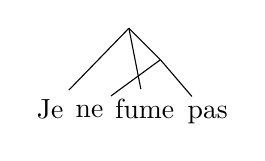
\begin{tikzpicture}

\node (je) at (0,0.07) {Je};
\node (ne) at (0.5,0.04) {ne};
\node (fume) at (1.2,0.08) {fume};
\node (pas) at (2,0) {pas};

\coordinate (nepas) at (1.4,0.7);
\coordinate (jefume) at (0.6,0.7);
\coordinate (all) at (1.0,1.1);

\draw (nepas) -- (ne);
\draw (nepas) -- (pas);
\draw (je) -- (all);
\draw (fume) -- (all);
\draw (all) -- (nepas);

\end{tikzpicture}
\caption{'non-projective' tree}\label{fig:struct3}
\end{figure}

Without attaching any rules to the structures, it is impossibly to quantify coverage of the set of structures, or the easy with which sentences can be disambiguated. For applications or empirical research, labels thus need to be considered (or learned).

\section{Translation Structures}

Even when assuming compositional grammars for two languages exist, it is still questionable whether it is possible to find a mapping between the two grammars. Of course, in theory we could just create a mapping that maps entire source structures to entire target structures, in practice, however, we cannot.\footnote{And if this were possible, we might as well just create a mapping that maps entire source sentences to entire target sentences and be done with it.} A mapping should thus map parts of structures to parts of structures, and combine these parts into a new structure (yielding a compositional construction of the translation). This section is structured similarly to the previous one: we start with a theoretical discussion of mappings, which is followed by a discussion of how compositional translation manifests itself in practice.
 
\subsection{Theory}

As compositionality of language, compositionality of translation is described in a principle:

\begin{quote}
\textbf{The Principle of Compositionality of Translation}\\
Two expressions are each others translation if they are built up from parts which are each other's translation, by means of translation-equivalent rules. (ref??)
\end{quote}

In other words, compositional translation takes place by identifying the compositional structure of the target language, mapping the syntactic rules to translation equivalent rules on the source side, and recursively determining the translation equivalence of the parts. Compositional translation is a very common method in translation between artificial languages \citep{janssen1996compositionality,janssen1998algebraic}. The translation from one logical language into another, or the translation the compiler performs when interpreting a programming language are all compositional. When considering a purely semantical compositional grammar, it seems that compositionality of translation should also hold for natural language, yet it is unclear if translation can actually be executed this way. We will discuss the main issues.

An important assumption that is underpinning the principle, is that in translation not only meaning, but also form should be preserved (as much as possible). In other words, it assumes that translation is literal. For artificial languages this property is straight-forward and useful, mostly because there are no a priori reasons to prefer a non-literal translation over a literal translation. In natural language, this assumption is more questionable. There are many occasions in natural language in which the assumption seems fairly applicable. It captures, for instance, the fact that `all ravens are black' is an adequate translation of `alle raven zijn zwart', while the logical equivalent `if something is not black it is not a raven' is not \citep{landsbergen1989power}. However, in practice a translator can have many reasons to prefer a free translation even if a more literal alternative is also available. In MT-systems, this issue is often ignored, which does not seem like a huge concession, given that the these systems are not (yet) focussing on literary translations, and the most literal translation is often a reasonably good, or at least acceptable translation.

Syntactic and lexical translational divergences form a second problem for compositional translation. Languages do not always express the same set of meanings, or express meanings in the same way. Even in languages of cultures that are quite similar, one can find a number of words that simply do not have an adequate translation in the other language (e.g., in translation between English and Dutch the words `gezellig' and `evidence' do not seem to have a clear equivalent in the other language), and even if the same meaning is expressed there are many syntactic phenomena in natural language that seem to be problematic for a compositional translation.  For example: different ways of role expression (e.g., `I like (obj)' and `\textcyr{mne nravitsa (subj)}') or syntactic mismatches (e.g., `woonachtig zijn' and its translation `reside' \citep{landsbergen1989power}).  The grammar rules and basic units can thus not simply be taken from a monolingual grammar, as there is no guarantee that the rules and basic units will have a translation equivalent rule or basic unit in the other grammar. The grammars must be constructed for translation, such that they are `attuned' \citep{rosetta1994compositional}. \cite{rosetta1994compositional} showed that previous mentioned examples do not necessarily stand in the way of compositional translation, by manually constructing a grammar for translation from English to Dutch, covering many non-trivial translation phenomena. However, their grammar consist of separate semantic and syntactic formalisms, which makes their case more complicated than the more direct structure mapping we are interested in for this thesis.

In summary, even when the existence of compositional structures for languages and literalness of translation is assumed, there is no guarantee that the structures of the two languages can be linked in a consistent fashion. Suitable compositional structures for a language might thus depend on which language it should be translated in. The nature of this problem suggests that if compositional syntactic structures for languages  can be constructed, they should have a strong semantic motivation.

\subsection{In Practice}

Compositional structures of translation are representation-wise very similar to compositional structures of language: they are tree representations that describe how the sentence was compositionally translated. The difference lies in the notion of parts: in compositional language structures, the parts were sequences of words that were combined through syntactic relations, while in compositional translation structures, the parts are defined through translation equivalence. Consider, for instance, the sentence pair (I give my little brother a ball, Ik geef mijn kleine broertje een bal), in which the translation equivalence is made explicit through linking the `parts' that were used in the translation. Note that if tree pairs are constructed as such through compositionality, every source node tree has an equivalent target node tree, the two resulting trees are thus isomorphic.

\begin{figure}[!ht]
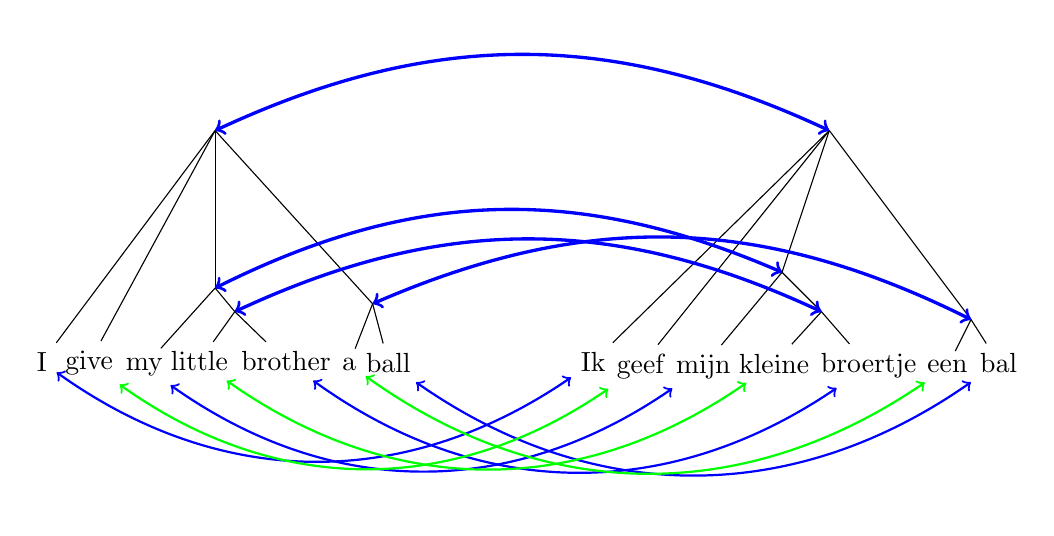
\begin{tikzpicture}


\node (I) at (1,0.06) {I};
\node (give) at (1.6,0.05) {give};
\node (my) at (2.3,0) {my};
\node (little) at (3.0,0.07) {little};
\node (brother) at (4.1,0.07) {brother};
\node (a) at (4.9,0.03) {a};
\node (ball) at (5.4,0.05) {ball};

\coordinate (toycar) at (5.6,0.7);
\coordinate (littlebrother) at (3.45,0.7);
\coordinate (mylittlebrother) at (3.2,1);
\coordinate (aball) at (5.2,0.8);
\coordinate (all) at (3.2,3);

\foreach \from/\to in {aball/ball, aball/a, littlebrother/little, littlebrother/brother, mylittlebrother/my, mylittlebrother/littlebrother, all/give, all/mylittlebrother, all/aball, all/I}
	\draw (\from) -- (\to);
	
\node (Ik) at (8,0.06) {Ik};
\node (geef) at (8.6,0) {geef};
\node (mijn) at (9.4,0) {mijn};
\node (kleine) at (10.3,0.04) {kleine};
\node (broertje) at (11.5,0.01) {broertje};
\node (een) at (12.5,0) {een};
\node (auto) at (13.15,0.05) {bal};

\coordinate (kleinebroertje) at (10.9,0.7) {};
\coordinate (mijnkleinebroertje) at (10.4,1.2);
\coordinate (eenauto) at (12.8,0.6);
\coordinate (alles) at (11,3);

\foreach \from/\to in {eenauto/auto, eenauto/een, kleinebroertje/kleine, kleinebroertje/broertje, mijnkleinebroertje/mijn, mijnkleinebroertje/kleinebroertje, alles/Ik, alles/geef, alles/mijnkleinebroertje, alles/eenauto}
	\draw (\from) -- (\to);	

\foreach \from/\to in {all/alles, mylittlebrother/mijnkleinebroertje, littlebrother/kleinebroertje, aball/eenauto}
	\draw[<->, bend left =25, very thick,blue] (\from) to (\to);

\foreach \from/\to in { broertje/brother,  mijn/my, Ik/I, auto/ball}
	\draw[<->, bend left =35, thick,blue] (\from) to (\to);

\foreach \from/\to in {een/a,  kleine/little, geef/give}
	\draw[<->, bend left =35, thick,green] (\from) to (\to);

\end{tikzpicture}

\caption{linked structures}\label{fig:transtrees}
\end{figure}

Unfortunately, the complexity of the given example is far below average. There is no translational divergence complicating the establishment of translation equivalence, the sentences have the same length, no reordering takes place,
and all translation equivalent sequences are contiguous. In fact, the target sentence is a word for word translation of the source sentence, which means that any source structure could be mapped to an isomorphic target structure through translation equivalence.

To establish isomorphism in harder cases, a phrasal approach is required. In Figure \ref{fig:phrasal}, a very simple example is given, of the translation of the three word phrase `a toy car' into the two word phrase `een speelgoedautootje'.

\begin{figure}[!ht]
\centering
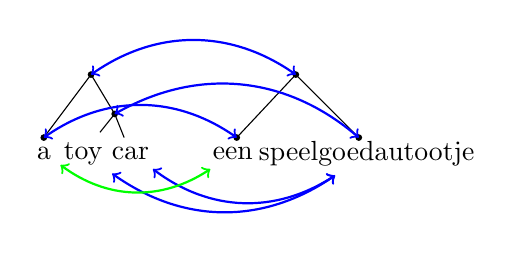
\begin{tikzpicture}

\node (a) at (0,0) {a};
\node (toy) at (0.5,0) {toy};
\node (car) at (1.1,0) {car};
\node (een) at (2.4,0) {een};
\node (auto) at (4.1,0) {speelgoedautootje};

\filldraw (0,0.2) circle (0.035);
\filldraw (2.45,0.2) circle (0.035);
\filldraw (4.0,0.2) circle (0.035);
\filldraw (0.9,0.5) circle (0.035);
\filldraw (0.6,1) circle (0.035);
\filldraw (3.2,1) circle (0.035);

\coordinate (toycar) at (0.9,0.5);
\coordinate (a_) at (0,0.2);
\coordinate (een_) at (2.45,0.2);
\coordinate (auto_) at (4.0,0.2);
\coordinate (all) at (0.6,1);
\coordinate (allnl) at (3.2,1);

\foreach \from/\to in {toycar/toy, toycar/car,all/toycar, all/a_, allnl/een_, allnl/auto_}
	\draw (\from) -- (\to);	

\foreach \from/\to in {auto/car,  auto/toy, a_/een_, toycar/auto_, all/allnl}
	\draw[<->, bend left =35, thick,blue] (\from) to (\to);

\draw[<->, bend left = 35, thick, green] (een) to (a);

\end{tikzpicture}
\caption{Phrasal translation equivalence}\label{fig:phrasal}
\end{figure}

From the previous two examples, it is not yet clear how such translation structures deal with reordering. It is important to realise that translation equivalence of two phrases does not imply that the order \textit{within} the phrases is identical. The phrases `una casa comoda' and `een comfortabel huis' are translation equivalent, even though the noun adjective order is not the same. Reordering by permuting the children in a parse tree is in practice quite powerful, although theoretically the fraction of reorderings that can be accounted for rapidly decreases with the length of the sentence \citep{satta2005some}.

Note that reordering amplifies the need of rules. Without them, it is impossible to always correctly guess the order of the leaf nodes of the target side tree.

\section{Combining Hypotheses}

We have discussed compositional structures for natural languages, we have discussed compositional translation structures, and we do now know what it means for them to coincide: the monolingual parts should have (contiguous) translation equivalent (contiguous) parts in the other sentence. There are often multiple compositional structures possible for source and target sides, depending on the intuitions of the creator of the structure. Furthermore, after establishing translation equivalence, there are often even more possible translation structures (... for the sentence pair in Figure \ref{fig:transtrees}), we have now thus arrived at the situation depicted in Figure  \ref{fig:comp2x}.

\begin{figure}[!ht]
\centering
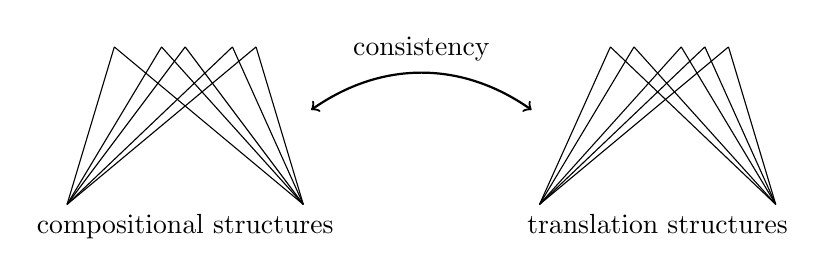
\begin{tikzpicture}

\coordinate (ss) at (1.5,0);
\node [below] at (ss) {compositional structures};

%\draw[] (0,0) -- node[below]{} (3,0);
\draw (0,0) -- (0.6,2) (3,0) -- (0.6,2);
%\draw (0,0) -- (0.9,2) (3,0) -- (0.9,2);
\draw (0,0) -- (1.2,2) (3,0) -- (1.2,2);
\draw (0,0) -- (1.5,2) (3,0) -- (1.5,2);
%\draw (0,0) -- (1.8,2) (3,0) -- (1.8,2);
\draw (0,0) -- (2.1,2) (3,0) -- (2.1,2);
\draw (0,0) -- (2.4,2) (3,0) -- (2.4,2);

\coordinate (ts) at (7.5,0);
\node [below] at (ts) {translation structures};

%\draw (6,0) -- (0.6,2) (9,0) -- (6.6,2);
\draw (6,0) -- (6.9,2) (9,0) -- (6.9,2);
\draw (6,0) -- (7.2,2) (9,0) -- (7.2,2);
%\draw (6,0) -- (7.5,2) (9,0) -- (7.5,2);
\draw (6,0) -- (7.8,2) (9,0) -- (7.8,2);
\draw (6,0) -- (8.1,2) (9,0) -- (8.1,2);
\draw (6,0) -- (8.4,2) (9,0) -- (8.4,2);

\coordinate (startarrow) at (3.1,1.2);
\coordinate (endarrow) at (5.9,1.2);
\node (t) at (4.5,1.7) [above]{consistency};

\draw[<->,bend left =35, thick] (startarrow) to (endarrow);

;\end{tikzpicture}
\caption{matching compositionality of translation and compositionality of natural language.}\label{fig:comp2x}
\end{figure}

We can find a set of structures according to which the sentence has been compositionally translated, we can find a set of structures that (possibly linguistically motivated) expresses the compositional structure of a sentence, but we do not know if it possibles to find consistency along these two sets. This topic is the main concern of this thesis.

\section{Empirically Studying Compositional Translation}

Thus far, we have discussed compositional translation on a practical yet unspecific level, as we have relied on intuition to determine both linguistic and translation equivalent parts (and structures). If compositional translation were to be used in an MT-model, however, means are needed to establish equivalences automatically and large scaled. The same holds, for empirical analyses of translation data (anders). In the current section, we will discuss these means, and the simplifications that are made in the process.

\subsection{Monolingual Compositionality}
\label{sec:depgram}

There are many monolingual grammar formalisms, few of which have parsers that can efficiently assign structures to large corpora of texts. The most common formalisms in MT are finite state machines, context free grammars, and dependency grammars. Although some cognitive researchers might disagree about the workings in the mind (ref rens?), the expressibility of finite state machines seems too weak to account for natural language. We will disregard them for the rest of this thesis. Constituency grammars have shown to be a quite suitable model for natural language, although language does not seem to be entirely context free \citep{shieber1987evidence}. Also, the labels of standard constituency grammars are based on the syntactic categories of words and phrases rather than being semantically motivated, which does seems suboptimal for translation. Although we will discuss some empirical work assessing the consistency of constituency grammars with translation data, in our own work we will solely focus on dependency grammars, which we will discuss elaborately in this subsection. Dependency grammars seem very suitable for the task at hand, as they are largely semantically motivated, and thus have potential to be consistent over language. We will shortly discuss the motivation and background of dependency grammars, give a formal definition and provide some clarifying examples.

\subsubsection{Background}

Contrary to phrase structure grammars, that establish relations between constituents of a sentence, a dependency grammar does not divide sentences in phrases. Rather, it is based on the idea that in a sentence all words but one depend on another word in the sentence, via a(n asymmetric) binary relationship that describes how the former word modifies or complements the latter. For instance, in the sentence `I really like writing my thesis', `my' depends on `thesis', as it complements it, and `really' depends on `like', which it modifies. Words can be said to have a valency, depending on how many dependents they need to be saturated (e.g., `like' would have a valency of two 2, as it needs both a subject and an object).

Although traditional dependency grammar (DG) has been used by linguists since the Middle Ages \citep{covington1990dependency}, modern DG is often seen as being created by \cite{tesniere1959elements}, whose cognitive motivation for it is worth citing:

\begin{quote}
The sentence is an organised whole; its constituent parts are the words. Every word that functions as part of a sentence is no longer isolated as in the dictionary: the mind perceives connections between the word and its neighbours; the totality of these connections forms the scaffolding of the sentence. The structural connections establish relations of dependency among the words. Each such connection in principle links a superior term and an inferior term. The superior term receives the name governor; the inferior term receives the name dependent. \citep[Translation:][]{ryan2013}
\end{quote}

The criteria for being a head-dependent pair are a mix of syntactic and semantic criteria \citep{nivre2005dependency}, and generally depend on the grammatical function the sentence or with respect to the word it depends on. Not all dependency grammars are identical in the relations they are considering, and their treatment of certain intuitively problematic constructions as coordination and conjunction \citep{nivre2005dependency}. In this thesis, we will follow the convention used in \cite{de2006generating}.

\subsubsection{Formally}

A dependency grammar is a quadruple $\langle R,L,C,F\rangle$, consisting of a set $L$ of terminal symbols (lexemes), a set $C$ of auxiliary symbols (lexical categories), a $R$ set of dependency rules over the auxiliary symbols $C$, and an assignment function $F : L\rightarrow C$.\citep{hays1964dependency,gaifman1965dependency}

A dependency structure of a sentence $s = w_1~\ldots~w_n$ generated by such a grammar can be seen as a directed acyclic graph $\mathcal{G} = \langle V, E\rangle$, in which $V = \{w_1, \ldots,w_n\}$ and $E$ is a set of edges such that $(w_i,w_j)\in E$ if and only if there is a dependency relation between $w_i$ and $w_j$. Furthermore, the graphs satisfies the following two criteria:
\begin{enumerate}
\item $\exists! w\in V \forall w'\in V (w,w')\notin E$ (rootedness)
\item $\forall w_1 w_2 w_3 \in V( (w_1,w_3)\negthinspace\in\negthinspace E \land (w_2,w_3)\negthinspace \in\negthinspace E ) \rightarrow w_1 = w_2$ (single-headedness)
\end{enumerate} 

In other words: a well-formed dependency structure is a tree. The edges of a dependency graph (or branches of the tree) can be labelled with the function of the dependent. An example of such a labelled dependency graph is depicted in Figure \ref{fig:depgraph}.

\begin{figure}[!ht]
\centering
\begin{dependency}[theme=simple]%[hide label]
\begin{deptext}[column sep=.5cm, row sep=.1ex]
%PRP\$ \& NN \& RB \&[.5cm] VBZ \& VBG \& NN \\
My \& dog \& also \& likes \& eating \& sausage \\
\end{deptext}
\deproot{4}{}
\depedge{2}{1}{poss}
\depedge{4}{2}{nsubj}
\depedge{4}{3}{xvmod}
\depedge{4}{5}{xcomp}
\depedge{5}{6}{dobj}
\end{dependency}
\caption{Dummy Dependency Graph, find other later}\label{fig:depgraph}
\end{figure}

A third criterion that is often used is projectivity, that prescribes a linear ordering of the nodes in the tree. Projectivity simplifies parsing (ref), as it reduces the space of possible dependency parses, but it is often argued that it deprives dependency grammar from its most important asset \citep{covington1990dependency,debusmann2000introduction}: the elegant method for handling discontinuous constituents (see Figure \ref{fig:npdeptree}). For fixed word order languages like English, in which phrases belonging together tend to stay together, projectivity is thus a reasonable criterion, but to account for languages in which there are less restrictions on the word-order (e.g., Russian, Latin) non-projectivity is often required to provide an intuitive analysis. An example of a non-projective in a otherwise fixed word-order language (Dutch) is depicted in Figure \ref{fig:npdeptree}.

\begin{figure}[!ht]
\centering
\begin{dependency}[theme=simple]%[hide label]
\begin{deptext}[column sep=.5cm, row sep=.1ex]
Ik \& weet \& dat \& hij \& me \& liet \& winnen\\
\tiny{I} \& \tiny{know} \& \tiny{that} \& \tiny{he} \& \tiny{me} \& \tiny{let} \& \tiny{win}\\
\end{deptext}
\deproot{2}{}
\depedge{2}{1}{}
\depedge{2}{6}{}
\depedge{6}{3}{}
\depedge{6}{4}{}
\depedge{6}{7}{}
\depedge{7}{5}{}
\end{dependency}
\caption{Non projective dependency graph. Provide some explanation}\label{fig:npdeptree}
\end{figure}

\subsection{Compositionality of Translation}
\label{sec:alignments}

To construct the set of translation structures, we need to be able to find the translation equivalent parts in a sentence pairs. In MT, this is done by means of of word-alignments (we have briefly seen them before while discussing the IBM word-based models): mappings from source to target words that describe which target words were involved in the translation of which source words (an example is given in Figure \ref{fig:alignment}). Word-alignments give rise to a straightforward notion of translation equivalence: two sequences of words are translation equivalent, if the words in the one sequence are translated only into words in the other sequence, and vice versa (we will later put this on a more formal footage).

As translation equivalent parts, word-alignments are not directly visible when looking at a sentence and its translation, and thus need to be learned. In this section, we will discuss the most common method to learn word alignments. We will start with the definition of a word-alignment, then briefly discuss the different type of word-alignments that exist, and how they can be obtained.

\begin{figure}[!ht]
\centering
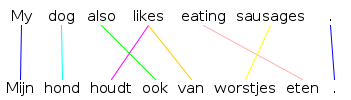
\includegraphics[scale=0.6]{alignment.png}
\caption{Word-alignments can be visualised in many ways. In this thesis, we will visualise alignments using lines, or arrows, where an arrow from source word $w_s$ to target word $w_t$ implies that $w_t$ was involved in the translation of $w_s$. The current figure shows a one-to-one alignment of the Dutch sentence `Na regen komt zonneschijn' and its translation `Auf regen folgt sonneschein'. The picture was generated by the alignment visualiser created by \cite{maillette2010visualizing}}
\label{fig:alignment}
\end{figure}


\subsubsection{Definition}

The precise definition of a word-alignment varies from paper to paper. Throughout this thesis we will use the following definition:

\begin{definition}[Alignment]\label{def:alignment}
Given a source sentence $s = s_0 \ldots s_n$ and its translation $t = t_0 \ldots t_m$, an alignment is a set $a \subseteq \{0,1,\ldots,n\} \times \{0,1,\ldots,m\}$ such that $(x,y)\in a$ iff $s_x$ is translated into $t_y$.
\end{definition}

In some definitions unaligned words are explicitly included in the alignment by adding an extra $NULL$ token to both source and target sets and including $(x,NULL)$ (or ($(NULL,y)$) in $a$ whenever word $x$ (or $y$) is unaligned. In our definition, unaligned words are not explicitly included: when a word $x$ is unaligned, this will be indicated by the absence of a word $y$ such that, respectively, $(x,y)$ or $(y,x)$, depending on whether $x$ was a source or target word. 


\subsubsection{Types of Word-alignments}

In the alignment in Figure \ref{fig:alignment}, every source word is aligned to exactly one target word and vice versa. Such an alignment is called a one-to-one alignment. It is also possible for source and target words to be aligned to more than one word, or to none at all, resulting in alignments that are one-to-many, many-to-one or even many-to-many. Another interesting property of the alignment depicted in Figure \ref{fig:alignment}, is that the target word order is identical to the source word order, resulting in an alignment in which none of the alignment links are crossing. Such an alignment is called monotone. The number of possible translation structures is largely determined by the complexity of the alignment, with rule of thumb: the simpler the alignment, the higher the number of possible structures. A summary of the restrictions corresponding to these different types of alignments is provided in Table \ref{table:alignments}.

\begin{table}[!ht]
\footnotesize{
\begin{tabular}{|ll|}
\hline
one-to-one & $\forall x\forall y \big( (x,y)\in y \to \forall z \big( (z,y)\in a \to z=x \land (x,z) \in a \to z=y \big ) \big ) $\\
&\\
one-to many & $\forall x\forall y \big( (x,y)\in y \to \forall z \big( (z,y)\in a \to z= x \big) \big) $\\
&\\
many-to-one & $\forall x\forall y \big( (x,y)\in y \to \forall z \big( (x,z)\in a \to z=y \big) \big ) $\\
&\\
many-to-many & - \\
&\\
monotone & $\forall w \forall x\forall y \forall z \big ( \left ( (x,y)\in a \land (w,z)\in a \land x < w \right ) \to y < z \big )$\\
\hline
\end{tabular}
}
\caption{Alignment types, restrictions}
\label{table:alignments}
\end{table}

\subsubsection{Translation Equivalence through Word-alignments}

Now that we have defined alignments, we can define translation equivalence. We will use the term `translation equivalent units' to refer to sequences that could have been `parts' in translation.

\begin{definition}[Translation Equivalence]
If $(s,t)$ is a pair of source and target sentences, and $A$ an alignment between $s$ and $t$. two sets of source and target words $w_s$ and $w_t$ are translation equivalent if and only if $$\forall x,y ( x\in w_s~(x,y)\in A \rightarrow y\in w_t \land x,y \in w_t~(y,x)\in A \rightarrow x\in A))$$
\end{definition}

The definition expresses the intuition that two sequences of words are translation equivalent, if the words in the first sequence are translated only into words in the second sequence, and vice versa. This definition does not includes a clause that states that such sequences need to be contiguous, a requirement that is often imposed in translation models as contiguous sequences are much easier to use in practice (and correspond to context freeness).

\subsubsection{Generating Word-alignments}

Even besides the fact that word-alignments are not visible in translation data, it is not always easy to establish which source words should be aligned to which target words. We will give two examples to illustrate this.

The first problematic cases are idiomatic expressions. The expression `Every cloud has a silver lining'  is synonymous with `Na regen komt zonneschijn', but it is unclear what would be a good alignment. Arguably, `has' should be aligned with `komt', as they are the only verbs in the sentence pair. However, when asking a bilingual Dutch and English speaker if `has' is a proper translation of `komt', the odds of obtaining a affirmative answer would be very slim. A more plausible alignment would align every Dutch word to every English words, indicated that the expression is translated as a whole. Such an alignment is called a phrasal alignment.

Problems also arise in the translation of function words, that do not have a clear translation equivalent in the other language. Consider, for instance, the word `does' in the sentence pair `John does not live here, John wohnt hier nicht'. As `does' has no clear translation in German, one might argue that it should be unaligned. However, the word seems to be connected with `live', so it could also be aligned with `wohnt'. A third option is to align `does' to `nicht', as it appeared with `not' when the sentence was negated.\citep[Example from][p.114]{koehn2008statistical}

\myparagraph{Manual Word-alignments}
In manually aligned corpora, the issues raised in the previous paragraph are often addressed by distinguishing sure alignment links and possible alignment links \citep{lambert2005guidelines}. The sure alignment links (indicated by the letter S) then represent unambiguous alignment links, while the possible alignment links (P) are less certain. Possible alignment links appear in case of phrasal translations, ambiguous translations, or in case two annotators disagree. 

There are very few manually aligned corpora, the only ones known to the author are presented in \cite{och2000improved}, \cite{graca2008building}, \cite{mihalcea2003evaluation} and \cite{pado2006optimal}, \cite{ahrenberg2000evaluation}. Short description of these corpora??
Manually annotating translation corpora is very labour intensive and none of these corpora are big enough to train models on. Rather, they are used to evaluate automatically generated word-alignments. A common metric used for this task is the alignment error rate (AER), that is defined as follows (ref?):

$$
\text{AER(S;P;A) = } - \frac{|\text{A}\cap\text{S}| + |\text{A}\cap\text{P}|}{|\text{A}| + |\text{S}|}
$$

A perfect score can thus be achieved by an alignment that has all the sure alignment points and some of the possible alignment points.

\myparagraph{Automatic Word-alignments}
Word alignments are established as a by-product for the word-based IBM models, and despite multiple efforts to improve on these alignments (e.g., refs), it is still common practice to use the alignments produced by the SMT toolkit used to train the IBM models \citep{och03:asc}. We will not discuss further methods for automatically word aligning corpora, but just briefly explain how the IBM alignments arise, and how many-to-many alignments are derived from them.

One step in the IBM models, is to learn a lexical translation model from a parallel corpus. If a word-alignment was directly visible from the data, this would be an easy task, as one could just count for each word how often it occurred in the text and how it was translated, and estimate a probability from these counts using relative frequency estimation (which happens to be the maximum likelihood solution) (anders). Conversely, given the lexical probability model, the most possible word-alignment could be estimated. Learning word-alignments and lexical probabilities from a parallel corpus can thus be seen as a problem of incomplete data, that can be addressed with the expectation maximization (EM) algorithm \citep{dempster1977maximum}, which works as follows:\begin{enumerate}
\item Initialize the lexical probabilities (often with uniform distributions).
\item Compute the most probable alignment from the lexical probabilities (expectation).
\item Recompute the lexical probabilities from the alignment found in the previous step (maximization)
\item Iterate steps 2 and 3 until convergence.
\end{enumerate}

\noindent Note that the use of such an algorithms means that the larger the corpus, the better the resulting alignments. It is thus not possible to align just one sentence.

In IBM model 1 and 2, the models that describe how the alignments depend on the lexical probabilities are sufficiently simple to exhaustively run the EM algorithm, and a (global) optimum is thus guaranteed to be found. To find the most probable alignments in the higher IBM models, stochastic hill climbing is used. Excellent examples of how the algorithm works on the IBM models can be found in \cite[p88-113]{koehn2008statistical}.

%Check order
The IBM models consider the sequence of target words as being generated by the source words one by one. Therefore, although source words can be aligned to more target words, every target word is aligned to at most one source word and the resulting alignments are thus many-to-one. However, many-to-many alignments are often desired, as they are very common in practice. Alignments used to train SMT models on are often created by running the IBM models in both directions, and combining the resulting alignments. The three most common methods of merging two alignments $A_1$ and $A_2$ are:\begin{enumerate}
\item Union: $A_1\cup A_2$, containing all links from both alignments. The recall of the union will be high (as it contains many links), but as it contains all faulty alignment links from both alignments too, the precision is often quite low.\footnote{Given a set of desired alignment points $A_{gold}$, recall and precision of an alignment $A$ are defined as follows:\\
$$\text{Recall = }\frac{|A \cap A_{gold}|}{|A_{gold}|} \text{\hspace{10mm}Precision = }\frac{|A \cap A_{gold}|}{|A|}$$
Given the nature of $A_{gold}$, precision and recall are not the common metrics used to evaluate word alignments.}
\item Intersection: $A_1\cap A_2$, containing only the links that occur in both alignments. The resulting alignment is thus a one-to-one alignment. Contrary to the union, the intersection of $A_1$ and $A_2$ (anders) will have a high precision, but a lower recall.
\item A more sophisticated method for combining alignments $A_1$ and $A_2$, is to first take the intersection, ending up with a selection of reliable alignment points, and then extend the alignment by adding neighbouring links and links $(i,j)$ for which holds that neither $e_i$ nor $e_j$ was aligned in the intersection \citep{och2000improved}, a heuristic called `grow-diag-final'. Pseudocode of this heuristic can be found in \cite{koehn2008statistical}.
\end{enumerate}

Most current MT models making use of alignments use the grow-diag-final method to obtain their alignments. The resulting alignments have a relatively high precision and recall \citep{och2000improved}, although they still contain several faulty alignment links. As mentioned before, several different alignment models that claim to have better alignment models have been reported (anders). Such methods are often based on .... list some things + references if you come across them. However, none of these methods has really found its way in the MT community. Besides the fact that it is hard to compare alignment methods across domains, it has been shown that improving alignment models does not necessarily result in better MT models... (anders, vind ref, kijk in wu alignment \cite{indurkhya2010handbook}).



\section{Foundations of Empirical Studies.}

We have now linked compositionality of language and compositionality of translation, and we have described means of generating compositional structures representing both of them. As we are dealing with real data produced by humans, we are not yet ready to start an empirical analysis, we have to make a few more assumptions. To appreciate empirical research, it is important to have a good picture of the simplifications that are made, and the influence they might have on the result. We will mention and discuss these assumptions, therewith describing the foundations of empirical research using translation data. At the end of this section, we will explicate a few concrete questions that can be addressed in the current framework.
%Given the size and nature of natural language, it is impossible to give an indisputable proof of the existence of such grammars, after all, how can one possibly show that a grammar covers all expressions that can be uttered by a human being. The theoretical question, however, evokes other questions of more practical nature, such as: (dit moet anders)
%
%\begin{itemize}
%\item How much of the structures generated by a grammar are respected by the translation data.
%\item If we assume linguistic structures on both source and target side are assumed, how far from bijective is the mapping needed to completely cover both trees.
%\item
%\end{itemize}


\subsection{Correctness of the Translation Data}

As empirical analyses are based on parallel corpora with text that are each others translation, it heavily relies on the correctness of these corpora. As these parallel texts were not designed as data for translation models, they might not be perfectly suitable for this purpose. When training MT models, infrequent mistakes in the data are generally not problematic, as they will receive a low probability. This is not the case with empirical analyses. There are three bottlenecks:

\myparagraph{1. Sentence level alignment.}
Aligning corpora on the sentence level is not as simple as it might seem. Texts are not always translated sentence by sentence. Short sentences may be merged or long ones broken up, and in some languages there are not even clear sentence delimiters \citep[p.55]{koehn2008statistical}. However, the techniques for sentence alignment are very good (ref??), it thus seems very reasonable to assume that the aligned sentences in the corpora do in fact have the same meaning.

\myparagraph{2. Correctness of translation. }
The texts are produced by humans, who sometimes make mistakes. To use the corpora, we have to assume that the aligned sentences are good translations of each other. Ref about quality??

\myparagraph{3. Translation is literal.}
One English sentence often has many translations in another language, as similar meanings can be expressed in multiple ways. For instance `jeg giver dig blomster' is a good Danish translation of `I give you flowers', but so is `jeg giver blomster til dig' (and the amount of rephrasing in this example is even rather minimal). Especially when one text is not a direct translation of the other text, but the two are, for instance, just separate reports of the same event, it might happen that sentences do have the same meaning, but are not very similar in form. In empirical analyses it is assumed that at least the vast majority of the translations in the corpora are rather literal.
 
\subsection{Word Alignments}

Also the previously discussed word-alignments are a bottleneck in empirical analysis of translation data. They are of crucial importance, as they are the mainstay for establishing translational correspondences, but are not always of high quality. Once again, MT-models do generally not suffer much from this fact, because the number of untrue alignment links is dwarfed by the number that is correct. For empirical research, false alignment links are quite problematic, as even one wrong link can have a huge effect on the space of possible translation trees. Empirical analyses therefore often use one of the few manually aligned corpora.

\subsection{Syntactic Parsers}

Not all models rely on linguistic information of the source and target languages, but if they do, automated parsers are required that provide this information. For English, high quality parsers are available, that make relatively little mistakes (refs?), although they may fail with rare phenomena. For other languages, this issue is often problematic.\\

Although statistical analysis of the corpora might provide more insight in the type of mistakes that are generally made, these types of mistakes will harm the outcome of an empirical analysis, making it more pessimistic than it would be if the data were perfect. It therefore seems sensible to see empirical analysis as an upper- or lowerbound (depending on the context), rather than an exact number.


\section{Empirical Analyses}

After having expounded the main assumptions of empirical research of translations, we can get to the concrete questions asked in such research, that are strongly related to the theoretical question: can we find compositional structures for two languages and mappings between them. There are several questions that might be answered by empirical research that closely relate to this theoretical question, that can be divided into more linguistically and more formally oriented questions, such as:

\begin{enumerate}
\item How much of the structures generated by a grammar are respected by translation data.
\item What is the minimum rule depth we need to find correspondences for entire syntactic source and target trees of a sentence pair?
\item What is the minimum branching factor that is needed to assign trees to all structures in the corpus.
\item What part of a corpus can be covered by binary translation trees?
\end{enumerate}

In this section, we will report the answers to these questions presented in research prior to this thesis.

\subsection{Linguistic Trees}

Several studies focus on the explanatory power of transforming linguistic parse trees, thus addressing the first two questions. Even though they are ran on different datasets, with different language pairs and use different criteria, they all find that linguistic parse trees do not coincide very well with translation corpora.

\subsubsection{Constituency grammars}

There are different ways of quantifying the suitability of monolingual linguistic parse trees. An often cited study is the one carried out in \cite{fox2002phrasal}. \citeauthor{fox2002phrasal} investigated how well linguistic phrases (i.e., constituents in a parse tree) stay preserved during translation from English to French. For her investigation, she used a manually aligned corpus created by \cite{och2000improved}, which contains 500 randomly selected sentences from the Canadian Hansard corpus. The manual alignments in this corpus are of type `sure' ($S$) and `possible' ($P$).\footnote{A more detailed description of the difference between these two alignment links can be found in Section \ref{sec:alignments}}. Fox counted the number of times the translation of distinct syntactic constituents (on the English side) overlapped or `crossed' (we will not five a formal definition of a `crossing', but provide an example in Figure \ref{fig:fox}. She concluded that crossings - even after filtering out phrasal translations that necessarily result in crossings - are too prevalent to ignore (on average 2.854 per sentence if all alignment links are considered).\footnote{With a manual analysis of the crossings in the constituency parses she showed that many of them are not due to the lac of phrasal cohesion, but are caused by errors in the syntactic analysis or rewording and reordering in the translation. Her analysis, however, included only the crossings of the S aligment links - the ones on which all annotators agreed and that were not ambiguous - that constitute just a small part of the total set of crossings.}


\begin{figure}[!ht]
\centering
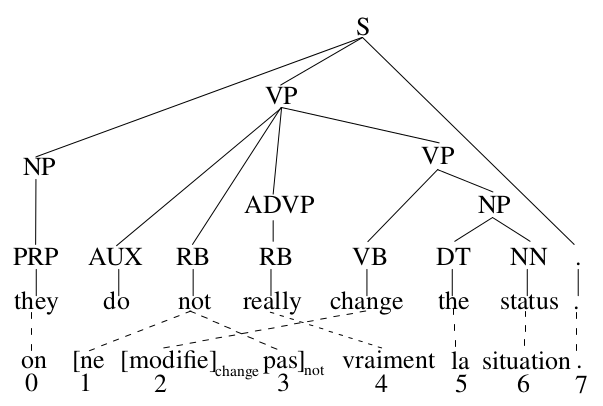
\includegraphics[scale=0.4]{crossing.png}
\caption{An example of a crossing according to \cite{fox2002phrasal}. Further explain.}\label{fig:fox}
\end{figure}

Her results are supported by others. \cite{galley2004s} focussed on the second question posed on the beginning of this Section. They generated constituency trees on the English side of the aforementioned Hansard corpus and tested how powerful a synchronous grammar should be to be consistent with the translation corpus. The power of the grammar was expressed in terms of the depth of the subtrees it generated, a standard CFG rule, that generates only single non-terminals, thus has depth 1. If rules of larger depth than 1 are needed, the non-terminal nodes of the syntactic source tree cannot be mapped bijectively to any target tree in a way consistent with the word-alignments. He found that only 19.4\% of the trees in the corpus could be entirely covered by one-depth-rules, and 85\% of the nodes (for the S alignments). Furthermore, he found that to cover the entire corpus with a grammar consistent with the allowed number of rule expansions should be no less than 17 for the S-alignments, and 23 for automatic alignments. For the English-Chinese corpus he analysed (FIBS, reference??), the coverage of low-expansion rules was even lower: 16.5\% (of the trees) for rules with a single expansion, and 100\% only with a maximum of 43\% expansions per rule.

\cite{khalilov2012statistical} confirmed the inadequacy of child-reordering in work that focusses on source reordering preliminary to translation. Using LRscore \citep{birch2010lrscore} as a measure of success, they concluded that permuting the children of nodes in a constituency tree is insufficient to reach a perfect permutation of source-words in English-Dutch and English-Spanish translation data, even when deleting up to 5 layers of nodes in the parse tree is allowed.\footnote{Their score for English-Spanish, however, is surprisingly high: around 94.}


\subsubsection{Dependency Grammars}

Not very much literature focusses on the consistency of dependency grammars with translation data, but some articles can be found on the matter. In her study about crossings, \citeauthor{fox2002phrasal} also devoted a section on dependency grammars. She observed that dependency parses are more cohesive than constituency grammars, with
2.714 crossings per sentence, compared to 2.854 for constituency grammars. A study that exclusively focusses on dependency parses was presented in \cite{hwa2002evaluating}. She investigated how well predicate argument structures agree between English and Chinese, addressing the validity of the Direct Correspondence Assumption.\footnote{Which expresses the intuition that there exists a mapping between the syntactic relationships in two sentences that are each others translation, and is thus directly allied to compositional translation} \citeauthor{hwa2002evaluating} evaluated the quality of Chinese dependency parses that were projected directly from English to Chinese through a manual word-alignment. The resulting parses ha a very low F-score (38.1), which is not surprising, as phrasal translations (multiple aligned words on source or target side) and unaligned target words always result in errors. \citeauthor{hwa2002evaluating} also observed this fact. They developed a small set of linguistically motivated rules, which boosted the F-score to 68.3, which is significantly higher, but still rather low. Also, it makes their work very specific, and hard to extend to other language pairs or contexts.

Another work along the same lines was presented by \cite{fung2006automatic}. \citeauthor{fung2006automatic} did not directly use dependency grammars, but learned cross-linguistic (English-Chinese) semantic verb frames. The learned argument mappings  had an accuracy of 89.3\%. It is unclear how their results compare to \citepos{hwa2002evaluating} results and dependency grammars in general, a fortiori because the exact nature of the learned semantic frames stays unclear.

\subsection{Formal Trees}

A second line of empirical research does not restrict source (or target) side trees to linguistic trees, but investigates the coverage of formal SCFG's. The majority of the empirical results on SCFG's focus on the coverage of binary trees \citep[e.g.,]{zhang2006synchronous,huang2009binarization}, or SCFG's in normal form \citep[e.g.,][]{sogaard2009empirical1,sogaard2009empirical2,sogaard2010can}. All concluded that the range of reordering phenomena occurring in real translation data are by far not as complicated as the worst case scenario sketched in \cite{satta2005some}.
%But also that...?

\cite{wellington2006empirical} seem to be the only one who compared their results with linguistically restricted parse trees. On several dataset (covering translation from Chinese, Romanian, Hindi, Spanish and French to English), he found that maximally 5\% of the alignments could not be explained by a completely binary tree, while the failure rate for binary trees that were constrained by monolingual parse trees on the English side climbed to 15\% for French/English to 61\% for Chinese/English. The failure rate they found for non constrained binary trees is much lower than the one found by \cite{simaan2013hats}, who reported a coverage of 71.46\% for the manual alignments of the Hansard corpus for trees with a maximal branching factor of 2. The coverage of binary trees for automatic alignments was even lower: 52.84\%. This difference between the results of \cite{wellington2006empirical} and \cite{simaan2013hats} is most likely due to a different treatment of alignment links: the latter authors used all alignment links in the dataset, while the former treated many-to-one alignment links disjunctively, focussing on lower bounds. \cite{simaan2013hats} also reported the coverage of non binarisable (permutation) trees, which is surprisingly enough not much higher: 72.14\% and 56.56\% for manual and automatic alignments, respectively.




%%%%%%%%%%%%%%%%%%%%%%%%%%%%%%%%%%%%%%%%%%%%%%%%%%%%%%%%%%%%%%%%%%%%%%%%%%%%%%%
% OWN WORK
%%%%%%%%%%%%%%%%%%%%%%%%%%%%%%%%%%%%%%%%%%%%%%%%%%%%%%%%%%%%%%%%%%%%%%%%%%%%%%%



\chapter{Own work}

It seems that in all these analyses, still no sufficient answer is found to the most general empirical question (anders): is it possible to match up compositionality of translation and compositionality of language, such that an entire translation corpus can be covered. In this thesis, we will address this question, where we hope to implicitly also find an answer to the question: are predicate argument structures preserved over language. To do so, we will consider a broad set of translation structures: all maximally compositional tree structures in which the non-terminal nodes are contiguous parts, and the discontinuous units are generated as terminals. In other words: all source structures that can be mapped to a target structure through a bijective mapping of the non-terminal nodes \citep[this set was previously defined in][]{simaan2013hats}. We will devise an algorithm for generating these structures in an easily accessible format that allows for investigation of the structures.

In this thesis, we will focus on the consistency of the translation structures with dependency grammars, that we believe have, given their semantic nature, potential for being consistent across languages. We will, making the same assumptions with regard to the translation data earlier investors did, investigate how well the translation structures cohere with dependency parses, and study the main causes of deviation of the translation structures of conventional linguistic syntax.

The structure of this chapter is similar to the structure of the previous chapter. First, we will define the set of translation structures we are considering. We will give some examples to hopefully provide a more intuitive feeling for this set, and explain how we will obtain and represent these structures (Section \ref{sec:transstr}). The next section addresses our compositional system of language (Section \ref{sec:compstr}). As we have discussed dependency parses quite elaborately earlier on, this section is of a more practical nature than the previous one. In Section \ref{sec:comb}, we will discuss how we will combine the two compositionality systems, giving formal definitions of consistency and examples to illustrate and motivate our procedures.


\section{Translation Structures}
\label{sec:transstr}

The set of translation structures considered in this thesis is the set as described in \cite{simaan2013hats}. We will first give a formal description of this set of structures (\ref{subsec:hats}), and then try to give a more intuitive description that illustrates the power of the set (\ref{subsec:intuition}). In the last part of this section (\ref{subsec:representation}, we will discuss the representational system we will use to describe and assess these structures.

\subsection{Formally}
\label{subsec:hats}

As the space of possible translation structures depends solely on the possible `parts' in translation, in the current set-up this space is completely determined by the positions of the source words and the positions they were mapped to, as described by the word-alignments. The current representation of alignments, as defined in Definition \ref{def:alignment}, is not optimal for devising translation structures. We will introduce, as far as this thesis goes, a change in notation. The alignment depicted in Figure \ref{fig:alignment2} will be referred to for clarification and explanation.

\begin{figure}
\centering
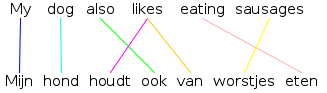
\includegraphics[scale=0.6]{alignment1.png}
\caption{A one-to-many alignment of the English sentence `My dog also likes eating sausages.' and its translation `Mijn hond houdt ook van worstjes eten'.%schrijf welke tool is gebruikt
\cite{maillette2010visualizing}
}\label{fig:alignment2}
\end{figure}

\subsubsection{Set-permutations}

Following \cite{simaan2013hats}, we will represent an alignment by an ordered sequence of sets, of which the $n$th element specifies to which target word the $n$th source word maps. In case of a one-to-one alignment, this sequence is thus a permutation of the target word-positions, while in more complex alignment some of the target positions may appear multiple times in the sequence, or not at all. We will refer to such a sequence describing an alignment with the term set-permutation, which is defined as follows:

\begin{definition}[Set-permutation]\label{def:sperm}
Given a source sentence $s = s_0 \ldots s_n$, its translation $t = t_0 \ldots t_m$, and an alignment $a$, let $a(i) = \{j~|~(i,j)\in a\}$ be the set with target positions that is linked to source position $i$. The set-permutation $\pi$ uniquely describing $a$ is defined as the ordered sequence of sets
$\langle a(0), \ldots, a(n) \rangle$
\end{definition}

\noindent The set-permutation $\pi = \langle\pi_0, ..., \pi_n\rangle$ describing the alignment depicted in Figure \ref{fig:alignment2} would thus be $\langle \{0\}, \{1\}, \{3\}, \{2,4\}, \{6\}, \{5\}\rangle$. 

\subsubsection{Translation Equivalence for Set-permutations}

With the altered definition for alignment, a new definition for translation equivalence is required. In the following definitions, we will assume that $\bigcup_{i=0}^{n} \pi_i$ constitutes a contiguous sequence of numbers (thus there are no unaligned words). Although this is not always the case in practice, such a situation can always be achieved by only numbering the aligned target positions that are aligned, effectively switching the position numbers to the left whenever an unaligned word is found, and can thus be assumed without loss of generality.

\begin{definition}[Translation Admissibility]\label{def:transadd}
Let $\pi = \pi_1 \ldots \pi_n$ be a set-permutation describing a sentence pair $(s,t)$, a subset $\{\pi_i,\ldots,\pi_j\}$ is translation admissible if and only if for every integer $x \in (\pi_i\cup \ldots \cup\pi_j)$ holds that $x \notin (\pi_0\cup \ldots \cup \pi_{j-1} \cup \pi_{i+1}\cup\ldots\cup \pi_n)$.
\end{definition}

\noindent The notion of translation admissible does not require contiguousness on either source or target side, which is desirable, as words are not necessarily translated into adjacent words in another language (for instance, in the running example `likes' translates into `houdt ... van'). A projective tree representation of a compositional translation, however, demands that that non-terminal cover contiguous subsequences in both source and target language, which leads to the following definition of translation part:

\begin{definition}[Translation Part]\label{def:transpart}
Let $\pi = \pi_1 \ldots \pi_n$ be a set-permutation describing a sentence pair $(s,t)$, a subset $\{\pi_i,\ldots,\pi_j\}$ is translation admissible if and only if $(\pi_i\cup \ldots \cup \pi_j)$ constitutes a contiguous range of integers (contiguousness on the target side), is a contiguous sequence in $\pi$ (contiguousness on the source side) and is translation admissible according to Definition \ref{def:transadd}.
\end{definition}

\noindent In the alignment depicted in Figure \ref{fig:alignment2} thus has 6 translation admissible sequences of length 1, 3 of length 2, 1 of length 3, 2 of length 4, 1 of length 5 and 1 of length 6 (see Figure \ref{fig:transequi}.

The number of translation parts in an alignment depends on the type of the alignment and is largest in case of a monotone alignment, that does not restrict the set of possible translation units at all. A completely monotone alignment of a sentence of $n$ words has $\frac{n\times n+1}{2}$ translation units. Note that unaligned words can cause exponential growth in the number of translation units.

\begin{figure}[!ht]
\begin{framed}
\small{
\begin{itemize}
\item \{0\} \hfill \{1\} \hfill \{3\} \hfill \{6\} \hfill \{5\} \hfill
\item \{\{0\},\{1\}\} \hfill  \{\{6\},\{5\}\} \hfill \{\{3\},\{2,4\}\}
\item \{\{1\},\{3\},\{2,4\}\}
\item \{\{0\},\{1\},\{3\},\{2,4\}\} \hfill \{\{3\},\{2,4\},\{6\},\{5\}\}
\item \{\{1\},\{3\},\{2,4\},\{6\},\{5\}\}
\item \{\{0\},\{1\},\{3\},\{2,4\},\{6\},\{5\}\}
\end{itemize}
}
\end{framed}
\caption{Translation units of alignment from \ref{fig:alignment2}}\label{fig:transequi}
\end{figure}


\subsubsection{Set-permutation Trees}

The set of compositional translation trees follows relatively straight-forwardly from the notion of parts: a compositional translation tree is a tree whose root span covers the entire sentence, and all of whose nodes correspond with translation equivalent units. To account for non-contiguous parts, nodes are allowed to expand in a combination of terminal and non-terminal nodes as well, provided that the terminals together constitute a translation admissible subset of the total sentence. A compositional translation tree will be defined in terms of allowed node expansions. If the top node of a tree covers the entire sentence, and all nodes are expanded as described in Definition \ref{def:exp1}, it recursively follows that all non-terminal nodes are translation parts and all leafnodes together constitute a translation admissible subset, and the tree is thus a compositional translation tree for the corresponding sentence.

\begin{definition}[Expansion of a translation part]\label{def:exp1}
Let $\pi = \langle \pi_0, \ldots,\pi_n\rangle$ be a set-permutation that constitutes a part of a translation. A allowed expansion of $\pi$ into parts is described by a segmentation of $\pi$ as an ordered set of indices $B = \{j_0 = 0, j_1, \ldots ,j_{m-1},j_m = n+1\}$ that segments $\pi$ into $m$ adjacent, non-overlapping and contiguous segments such that for all $0\leq i < m$ holds that the subsequence $\pi_{j_i}\ldots\pi_{j_{i+1}-1}$ is a new non-terminal node that is a translation part, or $\pi_{j_i}\ldots\pi_{j_{i+1}-1}$ constitutes a translation admissible sequence with ....
\end{definition}

Using Definition \ref{def:exp1}, a translation tree can be constructed top down, by recursively segmenting the entire sequence until only sequences of length 1 are left. Figure \ref{fig:alignment_tree} shows a possible alignment tree for the alignment from the running example: the sentence is firstly split into the two translation parts `my dog' and `also likes eating sausage', the former is then further split into two `my' and `dog', that also both constitute allowed translation parts. Also the right tree is further split up into translation parts, until the segmentation of `also likes' is reached, and no further division into allowed translation parts is possible. The phrase is therefore segmented into the non-terminal node covering part `also', and the leafnode covering the translation admissible word `likes'. Depending on its type, an alignment may have many different possible alignment trees. The current alignment has more than 40 different trees. The number of alignment trees can be exponential in the length of the sentence, if no restriction is placed on the branching factor of the nodes. Every alignment can be assigned at least one structure (the completely flat one).

\begin{figure}[!ht]
\centering
\Tree [.\{\{0\},\{1\},\{3\},\{2,4\},\{6\},\{5\}\} [.\{\{0\},\{1\}\} [.\{0\}  my ] [.\{1\} dog ] ] [.\{\{3\},\{2,4\},\{6\},\{5\}\} [.\{\{3\},\{2,4\}\} [.\{3\} also ] [.likes ] ] [.\{\{6\},\{5\}\} [.\{5\} eating ] [.\{6\} sausage ] ] ] ]
\caption{A possible alignment tree for the alignment of Figure \ref{fig:alignment} \label{fig:alignment_tree}}
\end{figure}

\subsubsection{Maximally Compositional Trees}

In this thesis, we will consider only a subset of the alignment trees we have just described: the ones that are maximally compositional in the sense that every node was expanded into a minimal number of child nodes (i.e.,the number of syntactic rules used in the sentence was maximal). The trees are thus minimally branching, if a node can expand into two parts, there will be no compositional translation tree in our set in which this node has more than 2 children.

Of course, there is a computational advantage to considering only minimally branching trees. Not only does it significantly reduce the space of trees to be considered (in case of the running example, 5 instead of 44), it also simplifies parsing, as the lower-rank rules that can be extracted from minimally branching trees  can be more efficiently treated by a parsing algorithm (ref?). Although these considerations are very relevant if a model were to be constructed from the
findings of this investigations, it seems that an empirical analysis assessing the underlying assumptions of models should not be primarily driven by computational issues. However, there are also theoretical advantages to considering only minimally branching trees. First of all, it secures the underlying system is indeed compositional. The set of all compositional translation trees contains many flat trees, that can under some perspective be seen as compositional (as compositionality is highly underspecified), but can not be seen as recursive or systematic. A grammar containing a separate rule for almost every sentence, specifying how the meaning can be derived from \textit{all of its words} does certainly not correspond with human intuitions about compositionality, not to mention the fact that such a grammar would be infinite. Considering only minimally branching trees solves this problem. Secondly, considering only expansions that are maximally compositional maximises the chance that generalisation to new data is possible (ref?): a rule that specifies how an argument can be combined with a predicate is more useful than a rule specifying how `I' can be combined with `like'. Minimum depth expansions are more probable to be applicable in new situations.

\subsection{Intuition}
\label{subsec:intuition}

In words, the set of structures considered in this thesis can be characterised by the following properties:
\begin{enumerate}
\item The structures are projective trees.
\item The non-terminal nodes in the tree correspond to subsequences that were possible parts in the translation, while sibling terminal nodes toghether constitute a translation admissible part, herewith respecting the strategy of compositional translation.
\item Nodes can have both non-terminal nodes and terminal children.
\item All nodes of the tree have a minimal branching factor.
\end{enumerate}

\noindent The set of structures considered is thus associated with a synchronous context-free grammar, in which expansion into the most general non-terminals is preferred over expansions into words, and phrasal translations are used only when necessary. This captures the intuition that even in complicated cases like syntactic divergence, the parts constituting the most important elements of the sentence are grossly the same, and the difference in syntactic structure is reflected only in a few words. We will provide some examples to elucidate this.

\begin{figure}[!ht]
\centering
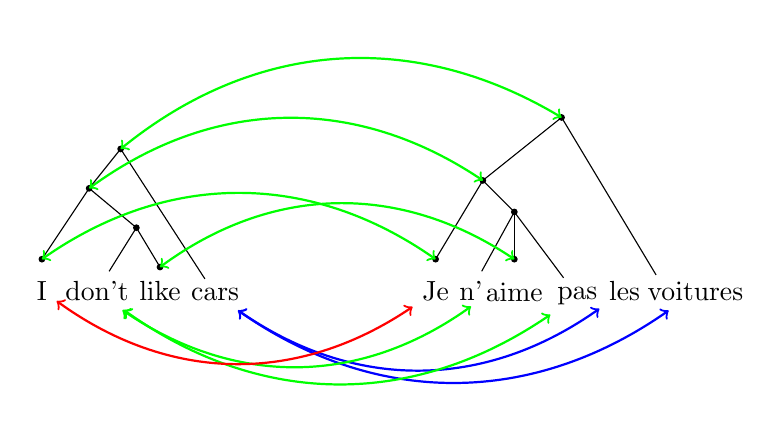
\begin{tikzpicture}
\draw node (I) at (0,0) {I};
\draw node (dont) at (0.7,0) {don't};
\draw node (like) at (1.5,0) {like};
\draw node (cars) at (2.2,-0.05) {cars};

\draw node (Je) at (5.0,0) {Je};
\draw node (n) at (5.45,0) {n'};
\draw node (aime) at (6.0,-0.02) {aime};
\draw node (pas) at (6.8,-0.07) {pas};
\draw node (les) at (7.4,0) {les};
\draw node (voitures) at (8.3,-0.01) {voitures};

\coordinate (Je_) at (5.0,0.4);
\coordinate (like_) at (1.5,0.3);
\coordinate (I_) at (0,0.4);
\coordinate (aime_) at (6.0,0.4);
\coordinate (naimepas) at (6.0,1);
\coordinate (dontlike) at (1.2,0.8);
\coordinate (Idontlike) at (0.6,1.3);
\coordinate (Jenaimepas) at (5.6,1.4);
\coordinate (lesvoitures) at (7.8,0.2);
\coordinate (all) at (1,1.8);
\coordinate (tout) at (6.6,2.2);
\coordinate (n_) at (5.45,-0.2);

\foreach \coordinate in {dontlike, like_, I_, Je_, aime_, Idontlike, all, tout, Jenaimepas, naimepas}
	\filldraw (\coordinate) circle (0.035);

\foreach \from/\to in {naimepas/aime_, naimepas/n, naimepas/pas, dontlike/like_, dontlike/dont, Idontlike/I_, Idontlike/dontlike, all/Idontlike, all/cars, Jenaimepas/Je_, Jenaimepas/naimepas, tout/Jenaimepas, tout/lesvoitures}
	\draw (\from) -- (\to);

\foreach \from/\to in {cars/voitures, cars/les}
	\draw[<->, bend left = -35, thick, blue] (\from) to (\to);

\foreach \from/\to in {dont/n_, dont/pas, tout/all, Jenaimepas/Idontlike, aime_/like_, Je_/I_}
	\draw[<->, bend left = -35, thick, green] (\from) to (\to);

\draw[<->, bend left = -35, thick, red] (I) to (Je);

\end{tikzpicture}
\caption{Translation of negation, French-English}\label{fig:nepas}
\end{figure} 


A famous example that is often taken as troublesome in MT (refs?) is the translation of (English) negation in the non-contiguous French `ne ... pas'. Figure \ref{fig:nepas} shows a compositional translation tree that accounts for such a translation in the system sketched in this thesis. The translation tree shows that `I dont like' is the translation of `Je n'aime pas', but also contains the information that `don't' is phrasally translated as `ne ... pas'. Removing the negation in the English sentence results in the grammatical English sentence `I like cars', removing its translation equivalent in the France sentence in its (almost) grammatical `Je aime les voitures'. 

An example containing syntactic divergence in translation between Russian and English is depicted in Figure \ref{fig:russian}. In Russian, `X has Y` is (communistically) translated as `with X is Y', the object in English is thus the subject in Russian. Figure \ref{fig:russian} shows how this is dealt with in a translation structure. Note that although this translation tree is easily extendible to longer sentences with the same construction. By expanding the non-terminal nodes it can also capture sentences like `the girl with the long blond hair has a very old car with broken windows'.

\begin{figure}[!ht]
\centering
\begin{tikzpicture}

\draw node (the) at (0,0.02) {The};
\draw node (girl) at (0.75,0) {girl};
\draw node (has) at (1.4,0.04) {has};
\draw node (a) at (1.9,0) {a};
\draw node (car) at (2.4,0) {car};
\draw node (y) at (4,0) {\textcyr{u}};
\draw node (girlr) at (4.9,-0.02) {\textcyr{devuxka}};
\draw node (is) at (6.1,0.02) {\textcyr{est\char126}};
\draw node (carr) at (7.5,0.04) {\textcyr{avtomobil}};

\coordinate (thegirl) at (0.4,0.6);
\coordinate (acar) at (2.1,0.6);
\coordinate (thegirlhas) at (0.8,1);
\coordinate (all) at (1.4,1.5);
\coordinate (carr_) at (7.5, 0.3);
\coordinate (girlr_) at (4.9,0.3);
\coordinate (girlhas) at (4.9,0.8);
\coordinate (allr) at (5.9, 1.2);


\foreach \coordinate in {thegirl, acar, thegirlhas,all,carr_, girlr_, girlhas, allr}
	\filldraw (\coordinate) circle (0.035);

\foreach \from/\to in {thegirl/girl, thegirl/the, acar/a, acar/car, thegirlhas/thegirl, thegirlhas/has, all/thegirlhas, all/acar, girlhas/girlr_, girlhas/y, girlhas/is, allr/girlhas, allr/carr_}
	\draw (\from) -- (\to);

\foreach \from/\to in {the/girlr, girl/girlr}
	\draw[<->, bend left = -35, thick, blue] (\from) to (\to);

\foreach \from/\to in {has/y, has/is, allr/all, girlhas/thegirlhas, carr_/acar, girlr_/thegirl}
	\draw[<->, bend left = -35, thick, green] (\from) to (\to);

\foreach \from/\to in {a/carr, car/carr}
	\draw[<->, bend left = -35, thick, red] (\from) to (\to);


\end{tikzpicture}
\caption{Translation of possession, Russian-English}\label{fig:russian}
\end{figure}

The system is on some level thus very similar to a standard HPB model as presented by \cite{chiang2005hierarchical}. The major differences reside in rule selection, and the emphasis on exploring recursivity past the lexical level, which was underrepresented in Chiang's model, as only two glue rules were used.

\subsection{Representation and Generation}
\label{subsec:representation}

To study sets of translation structures, means to generate them are necessary. Hence, a suitable representation needs to be found, as generating and storing all trees separately would be both time and space consuming, and would impede a flexible search through them. We will represent the set of trees by a context-free grammar with spans as non-terminal nodes, that describes the allowed expansions of each span and uniquely generates the entire parse forest of the given sentence. An example is given in Figure \ref{fig:grammar}.

\begin{figure}[!ht]\begin{framed}
\small{
\begin{tabular}{llllll}
(0-6] $\rightarrow$ (0-1]  (1-6] && (4-6] $\rightarrow$ (4-5]  (5-6] && (0-1] $\rightarrow$ My\\
(0-6] $\rightarrow$ (0-2]  (2-6] && (0-4] $\rightarrow$ (0-1]  (1-4] && (1-2] $\rightarrow$ dog\\
(0-6] $\rightarrow$ (0-4]  (4-6] && (0-4] $\rightarrow$ (0-2]  (2-4] && (2-3] $\rightarrow$ also\\
(1-6] $\rightarrow$ (1-4]  (4-6] && (1-4] $\rightarrow$ (1-2]  (2-4] && (4-5] $\rightarrow$ eating\\
(1-6] $\rightarrow$ (1-2]  (2-6] && (0-2] $\rightarrow$ (0-1]  (1-2] && (5-6] $\rightarrow$ sausages\\
(2-6] $\rightarrow$ (2-4]  (4-6] && (2-4] $\rightarrow$ (2-3] likes\\
\end{tabular}
\caption{The grammar generating the translation tree forest for the sentence
`My dog also likes eating sausages', with set-permutation $\langle _0\{0\}_1,~ _1\{1\}_2,~ _2\{3\}_3,~ _3\{2,4\}_4, ~_4\{6\}_5,~ _5\{5\}_6\rangle$ would be (the subscripts indicating the span annotation, which is left exclusive and right inclusive)}\label{fig:grammar}
}
\end{framed}
\end{figure}

The allowed expansions were found with an algorithm similar to \citepos{dijkstra1959note} shortest path algorithm, that was adapted to be more efficient given the extra knowledge of the alignment graph (Algorithm \ref{alg:shortest paths}).

\begin{algorithm}[!ht]
\caption{Shortest Paths}\label{alg:shortest paths}
\begin{algorithmic}
\STATE \textbf{Input:} A graph $G = (V,E)$ describing an alignment and two vertices $i$ and $j$ for which $(i,j)\in E$ is true.
\STATE \textbf{Output:} All non-trivial shortest paths from $i$ to $j$
\STATE \textit{\#Initialization}
\STATE visited = $\emptyset$, depth = $0$, paths = $\{j\}$
\STATE $\forall n\in\mathbb{N}:$ reachable(n) = $\emptyset$; reachable($0$) = $\{j\}$
\STATE depth\_finished = False
\STATE \textit{\# Start backwards search through graph}
\WHILE{not depth\_finished or $i\notin$ visited}
	\WHILE{reachable(depth) $\neq\emptyset$}
		\STATE depth\_finished $\leftarrow$ False
		\STATE current\_node $\leftarrow N$ an arbitrary element $v$ from reachable(depth)
		\STATE reachable(depth) $\leftarrow$ reachable(depth) $-$ $\{$current\_node$\}$
		\FOR{ ($l$,current\_node) $\in E$}
			\IF{$l\notin $visited $\cup$ reachable(depth) \AND depth $\neq 0$}
				\STATE reachable(depth+1) $\leftarrow$ reachable(depth+1) $\cup$ $\{l\}$
				\FOR{path (current\_node,\ldots, $j) \in$ paths}
					\STATE path $\leftarrow$ ($l$,current\_node,\ldots, $j)$
				\ENDFOR
			\ENDIF
		\STATE visited $\leftarrow$ visited $\cup$ $\{l\}$
		\ENDFOR
	\STATE depth\_finished $\leftarrow$ True
	\STATE depth $\leftarrow$ depth+1
	\ENDWHILE
\ENDWHILE
\STATE \textbf{Return} paths
\end{algorithmic}
\end{algorithm}


\section{Compositional Structures}

The compositional system for language we will use in this thesis is the dependency grammar, as was already indicated in Chapter \ref{ch:empirical}. In this chapter, we have argued for the suitability of dependency grammars as translation minded compositional system of language, gave some background information, and provided a formal description. A short recap: dependency structures describe the relation between words, instead of describing a hierarchical structure between phrases, aiming to capture the cognitive perception of sentences in the human brain. Dependency structures can be seen as predicate arguments structures of sentences, that are highly semantically motivated.

\subsection{Formally}

A rather formal description of dependency grammars was already given, we will use this subsection to sharpen notational affairs and define dependency parses as they are used in our experimental part. We will define a dependency tree as a set of relations, holding between the (positions of the) words of the sentence:

\begin{definition}[Dependency structure]
A dependency structure of a sentence $s = w_0\cdots w_n$ is a set of dependencies $D = \{ (i,j) |$ there is a dependency arrow from word $w_i$ to word $w_j \}$. 
\end{definition}

There are many conditions that can be imposed on $D$ \citep{de2006generating}, of which in this thesis the most common ones will used\begin{enumerate}
\item When seen as a relation, $D$ constitutes a single-headed a-cyclic graph in which the words in $s$ are the nodes. (tree-constraint)
\item When the words are placed in the original order, the branches of the dependendency tree do not cross. (projectivity)
\end{enumerate}

The span of a word according to a dependency tree is defined as follows:

\begin{definition}
If $T_d$ is a dependency tree for $s$, $w$ is a word in $s$ and $i$ and $j$ are the maximum and minimum positions, respectively, that can be reached from $w$ by following the directed dependency arrows. Then span($w$) = $[i,j]$. 
\end{definition}

\subsection{Generation and Representation}

To assign dependency structures to sentences, we used the Stanford Dependency Parser, that can be downloaded from their website, as well as used online  \citep{de2006generating}. The parser provides 5 variants of a typed dependency representation, of which the most basic one corresponds to the earlier imposed conditions on dependency structures. An example dependency parse as generated by the parser is depicted in Figure \ref{fig:deptree1}.

\begin{figure}[!h]\label{fig:deptree1}
\centering
\begin{dependency}[theme=simple]%[hide label]
\begin{deptext}[column sep=.5cm, row sep=.1ex]
%PRP\$ \& NN \& RB \&[.5cm] VBZ \& VBG \& NN \\
My \& dog \& also \& likes \& eating \& sausage \\
\end{deptext}
\deproot{4}{}
\depedge{2}{1}{poss}
\depedge{4}{2}{nsubj}
\depedge{4}{3}{xvmod}
\depedge{4}{5}{xcomp}
\depedge{5}{6}{dobj}
\end{dependency}
\caption{Stanford Dependency Tree}
\end{figure}

Say something about stanford dependency parsers not including punctuation


Formally, dependency grammars are not interpreted as a compositional grammar, as they do not postulate the existence of non-terminal syntactic categories, and therefore do not explicitly specify how a sentence was built up from its parts. However, dependency graphs do give rise to an hierarchical structure that specifies from which smaller parts the sentence was composed. For instance, the dependency graph depicted in Figure \ref{fig:deptree1} tells us that `likes' is the head word of the sentence, and that the sentence is composed of 4 parts: the head `likes', its modifier `also', its noun subject whose head is `dog' and the open clausal complement whose head is `eating'. The complement and subject are further divisible in `My' and `dog', and `eating' and `sausage', respectively. As the tree is projective, all parts are continuous. Also the graph in Figure \ref{fig:depgraph} prescribes an hierarchical structure: it is composed of the subject `I', the headword `know', and the phrase headed by `liet', that is in its turn built up from its head `liet', `dat', `hij' and the discontinous phrase `me winnen'. Such an hierarchical structure can not be captured by a phrase structure grammar.

\section{Combining Translation Structures and Dependency Parses}

To combine dependency parses and translation structures, means need to be find to quantify consistency and similarity between them. We have arrived at the situation depicted in Figure \ref{fig:depshats}.

\begin{figure}[!ht]
\centering
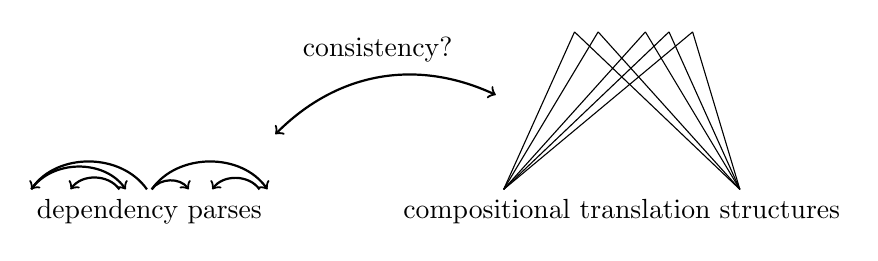
\begin{tikzpicture}

\coordinate (ss) at (1.5,0);
\node [below] at (ss) {dependency parses};

\draw[->,bend right = 55,thick] (1.47,0) to (0,0);
\draw[->,bend left = 55, thick] (1.53,0) to (3,0);
\draw[->,bend left = 55, thick] (0.0,0) to (1.2,0);
\draw[->,bend right = 55,thick] (1.12,0) to (0.5,0);
\draw[->,bend left = 55, thick] (1.53,0) to (2.0,0);
\draw[->,bend right = 55,thick] (2.9,0) to (2.3,0);

\coordinate (ts) at (7.5,0);
\node [below] at (ts) {compositional translation structures};

%\draw (6,0) -- (0.6,2) (9,0) -- (6.6,2);
\draw (6,0) -- (6.9,2) (9,0) -- (6.9,2);
\draw (6,0) -- (7.2,2) (9,0) -- (7.2,2);
%\draw (6,0) -- (7.5,2) (9,0) -- (7.5,2);
\draw (6,0) -- (7.8,2) (9,0) -- (7.8,2);
\draw (6,0) -- (8.1,2) (9,0) -- (8.1,2);
\draw (6,0) -- (8.4,2) (9,0) -- (8.4,2);

\coordinate (startarrow) at (3.1,0.7);
\coordinate (endarrow) at (5.9,1.2);
\node (t) at (4.4,1.5) [above]{consistency?};

\draw[<->,bend left =35, thick] (startarrow) to (endarrow);

\end{tikzpicture}
\caption{New situations: finding consistency between dependency parses and compositional translation structures}\label{fig:depshats}
\end{figure}

\noindent In this section, we will define coherence between dependency parses and compositional translation structures. In particular, we will define two methods to determine if a dependency parse is respected by a compositional translation tree,  and a recursive procedure for assigning a similarity score to compositional translation trees accordingly. 

\subsection{Direct Similarity}

Intuitively, a compositional translation tree is consistent with a dependency tree if they prescribe the same parts. An obvious similarity choice would thus be F-score (ref?), according to which the output of syntactic constituency parsers is evaluated. However, as we are comparing with dependency relations between words, it seems just as important that the parts are correctly combined, which is accounted for in our new definition of consistency. 

\begin{definition}[Consistency between Dependency relation and Alignment Tree]\label{def:depHAT}
Let $s = w_1 w_2 \dots w_n$ be a sentence, and $D = \{ (i,j) |$ there is a dependency arrow from word $w_i$ to word $w_j \}$ a set of dependencies describing a dependency tree for $s$. Let span($j$) be the range $[m,n]$ in which $m$ and $n$ are the maximum and minimum position that can be reached from $w_j$ by following the directed dependency arrows, respectively. A dependency relation $(i,j)$ is said to be respected by an alignment tree $T$ over $s$ if and only if there is a node in $T$ of which both $[i,i]$ and span($j$) are children.
\end{definition}

\noindent This consistency definition expresses the intuition that a predicate and its arguments are all generated one syntactic rule, and should thus be children of the same node. A dependency relation is respected by a compositional translation tree if the head and the entire phrase the dependent is heading are siblings in the tree.

\subsection{Deeper Similarity?}

The type of consistency defined in Definition \ref{def:depHAT} is very direct, and might assign many trees that seem perfectly in line with dependency parses a rather low score, due to different types of recursivity. Dependency structures are created by linguists, and although they certainly have a generality too them, they are not constructed to be \textit{maximally} recursive, as the set of used translation structures. We will give two examples to illustrate this.

Firstly, consider the sentence `I give you flowers', which contains one predicate (`give') with three arguments (the subject `I', the object `flowers' and the indirect object `you'). Its Dutch translation `Ik geef jou bloemen' has exactly the same predicate argument structure \textit{and} word-order, whereby the branching factor in any of its HATs will not exceed two. However, a maximum score can only be obtained by a tree in which `I', `give', `you', and `flowers' are siblings, whose mother will have a branching factor of (at least) four. Even though the translation of this sentence seems perfectly compositional, no HAT will thus obtain the maximum score, because the dependency structure is not minimally branching.

A second example, that is more related to translational divergence, arises when two arguments are translated into one (which happens, e.g., when arguments are translated as pre- or suffixes, when verbs do not require a subject or when spaces are emitted). Consider for instance the sentence 'Can you give me the salt' and its Italian translation 'puoi passarmi il sale'. Once again, the predicate-argument structure of the sentence is well preserved. However, the dependency parse prescribes that `the salt', `can' and `you' should be siblings of `give', which will be the case in none of the HATs over $\{\{0\},\{0\},\{1\},\{1\},\{2\},\{3\}\}$, as `give' and `me' are together translated into `passarmi', and `can you' into `puoi'.

To account for this discrepancy between maximally recursive alignment structures and dependency parses, we allow a predicate to combine with its arguments 'one-by-one', which would allow both given examples to get a maximal score. A dependency relation is thus respected by a compositional translation structure if the phrase headed by the dependent is siblings with the head itself, or the head plus arguments the head earlier combined with, which is defined in Definition \ref{def:depHAT2}.

\begin{definition}[Consistency2]\label{def:depHAT2}
Let $s = w_1 w_2 \dots w_n$ be a sentence, and $D = \{ (i,j) |$ there is a dependency arrow from word $w_i$ to word $w_j \}$ a set of dependencies describing a dependency tree for $s$. Let span($j$) be the range $[m,n]$ in which $m$ and $n$ are the maximum and minimum position that can be reached from $w_j$ by following the directed dependency arrows, respectively. Let $(i,j)$ be a dependency relation in $D$, and let $l_1,\ldots,l_n$ and $r_1,\ldots r_k$ be the left and right dependents of $i$, respectively, for which holds that $r_k < j$ or $l_1 > j$. A dependency relation $(i,j)$ is said to be respected by an alignment tree $T$ over $s$ if and only if one of the following three conditions is true: \begin{enumerate}
\item There is a node in $T$ f which both $[i,i]$ and span($j$) are children.
\item $\exists x$  and a node in $T$ of which span($l_x\ldots l_n~i~\ldots r_1 r_k$) and span($j$) are both children.
\item $\exists x$  and a node in $T$ of which span($l_1\ldots l_n~i~r_1\ldots r_x$) and span($j$) are both children.
\end{enumerate} 
\end{definition}


\subsection{Scoring Trees}

The (not yet normalised) score of a compositional translation tree can now be recursively defined as follows:

\begin{definition}[Scoring]
Let $s = w_1 w_2 \dots w_n$ be a sentence, and $D = \{ (i,j) |$ there is a dependency arrow from word $w_i$ to word $w_j \}$ a set of dependencies describing a dependency tree for $s$. Let $d_{i,j}$ be the set of relations that could make $(i,j)$ true in $T$, let $D'$ = $\{d_{i,j}| (i,j)\in D\}$. Let $H$ be an alignment tree for $s$. The (unnormalised) score of $H$ with $D$ is now defined as the score of its highest node $N$:

$$
E(N_a,D) = \sum_{c\in C_{N_a}} E(c,D)+ \sum_{c_1\in C_{N_a}} \sum_{c_2\in C_{N_a}} B(c_1,c_2)
$$

\noindent With base case $E(N,D) = 0$, $B(c_1,c_2) = 1$ iff  $(c_1,c_2)\in D'$, and $C_N$ the set of child nodes of $N$.

The score can be normalised by dividing by $|D|$.
\end{definition}

An example is given in the next subsection.

\subsection{Example}

We will provide an example for scoring the similarity between a compositional translation structure and a dependency parse according to direct similarity. Consider once again the dependency depicted in Figure \ref{fig:deptree1}. The set of dependencies $D$ is:

$$ \{ (0,4), (2,1), (4,2), (4,3), (4,5), (5,6) \}.$$


\noindent As direct similarity is used as consistency measure, $d_{i,j}$ = $[i,i], span(j)]$, thus we have:

$$D' = \{([1,1],[2,2]), ([4,4],[1,2]), ([4,4], [3,3]), ([4,4],[5,6]), ([5,5],[6,6])\}$$

\noindent The following tree (which is not maximally recursive) would receive the optimal score of 5/5, as all the 5 dependencies are present in the tree:\\

\Tree [.{[}1,6] [.{[}1,2] [.{[}1,1] my ] [.{[}2,2] dog ] ] [.{[}3,3] also ] [.{[}4,4] likes ] [.{[}5,6] [.{[}5,5] eating ] [.{[}6,6] sausage ] ]  ]

\noindent While the tree (also not maximally recursive)

\Tree [.{[}1,6] [.{[}1,2] [.{[}1,1] my ] [.{[}2,2] dog ] ] [ [.{[}3,3] also ] ] [.{[}4,6] [.{[}4,4] likes ] [.{[}5,6] [.{[}5,5] eating ] [.{[}6,6] sausage ] ] ] ] 

\noindent receives a slightly lower score of 3/5 as we miss dependencies (likes, also) and (likes, dog).



\chapter{Results}

We have ....
In this chapter, we will discuss the results of the automatic analysis of the translation data, and manually analyse these. (?)
This chapter is structured as follows. In Section \ref{sec:data}, we will start with a description of the data we have used for our analyses .. blablabla In Section \ref{sec:results1}, we will  discuss our results on the automatically aligned corpora

We will start with a description of our data, and the exact tools used to blablabla. In section ... blablabla





\section{Data}
\label{sec:data}

We will give a description of our data and the alignments blabla

\subsection{Corpora}

We ran our tests on several corpora, that were either aligned automatically or manually. The translation direction considered was always from English to foreign language. The English side of the corpus was parsed with the Stanford dependency parser \citep{de2008stanford} using newlines as delimitation, as to respect the sentence alignment of the corpora, to obtain basic typed dependencies of the sentences. Note that the dependency parser used does not take into account punctuation, which sometimes complicates the analysis. We will now give a short description of the data used, a summary can be found in \ref{tab:datasets}.

\subsubsection{Automatically Aligned Corpora}
The larger, automatically aligned, corpora for English-French, English-Dutch and English-German consisted of 200.000 sentences drawn from the Europarl corpus (ref?), while the English-Chinese corpus used consisted of 200.000 sentences from .... . The corpora were all automatically aligned with the Giza++ tool (ref) designed by IBM, using the previously described `grow-diag-and-final'-heuristic, with 4 iterations on model 1, 3 on the hmm model, model 3 and model 4.


\subsubsection{Manually Aligned Corpora}
We attempted to further analyse the consistency between dependency parses and translation data by also testing manually aligned data, that contain more reliable alignment links and are thus more suitable for empirical analysis. As far as the author knows, no manually aligned corpora for translation from English to Dutch are available, we did find two manually aligned corpora for translation from English to French, and one for translation from English to German. In addition, we analysed  2 new language pairs, of which manually aligned corpora were available: English-Portuguese and English-Spanish. The data were manually aligned by \cite{graca2008building} (en-fr, en-sp and en-pt), \cite{pado2006optimal} (en-de) and \cite{och2000improved} (en-fr).

\begin{table}
\begin{tabular}{llllll}
Language & Corpus & & Section & Aligned\\
\hline
English - Dutch & Europarl & & automatic \\
English - French & Europarl & automatic \\
English - German & Europarl & automatic \\
English - Chinese & & & automatic \\
English- French & Hansard & & manual\\
\end{tabular}
\caption{Datasets}\label{tab:datasets}
\end{table}


We parsed the English side of the corpus with the Stanford dependency parser \citep{de2008stanford} using newlines as delimitation, to obtain basic typed dependencies of the sentences. Note that punctuation is thus not taken into account.

\section{Direct Similarity}



\begin{table}[!h]
\centering
\begin{tabular}{l|ccc}
& \multicolumn{3}{c}{Multi-column}\\
Language pair & |s| < 10 & |s| < 20 & |s| < 40\\
\hline
English-Dutch & 0.47 & 0.42 & 0.40 \\
English-French & 0.45 & 0.42 & 041 \\
English-German & 0.44 & 0.41 & 0.38 \\
English-Chinese & 0.59 & 0.48 & 0.42\\
\end{tabular}
\caption{Results Experiment 1, automatic alignments}\label{tab:scores1}
\end{table}

\appendix
\chapter{Implementation}
\label{appendix:impl}

\chapter{Manual Analysis}
\label{appendix:analysis}



\bibliography{thesisDH}
\end{document}